% ==========================================
% BAB II TINJAUAN PUSTAKA
% ==========================================
\cleardoublepage
\chapter{TINJAUAN PUSTAKA}
\label{chap:II}

\section{Peta Literatur}
\label{sec:II.1}

Berikut adalah peta literatur yang digunakan dalam penelitian ini.
\begin{figure}[htbp]
\centering
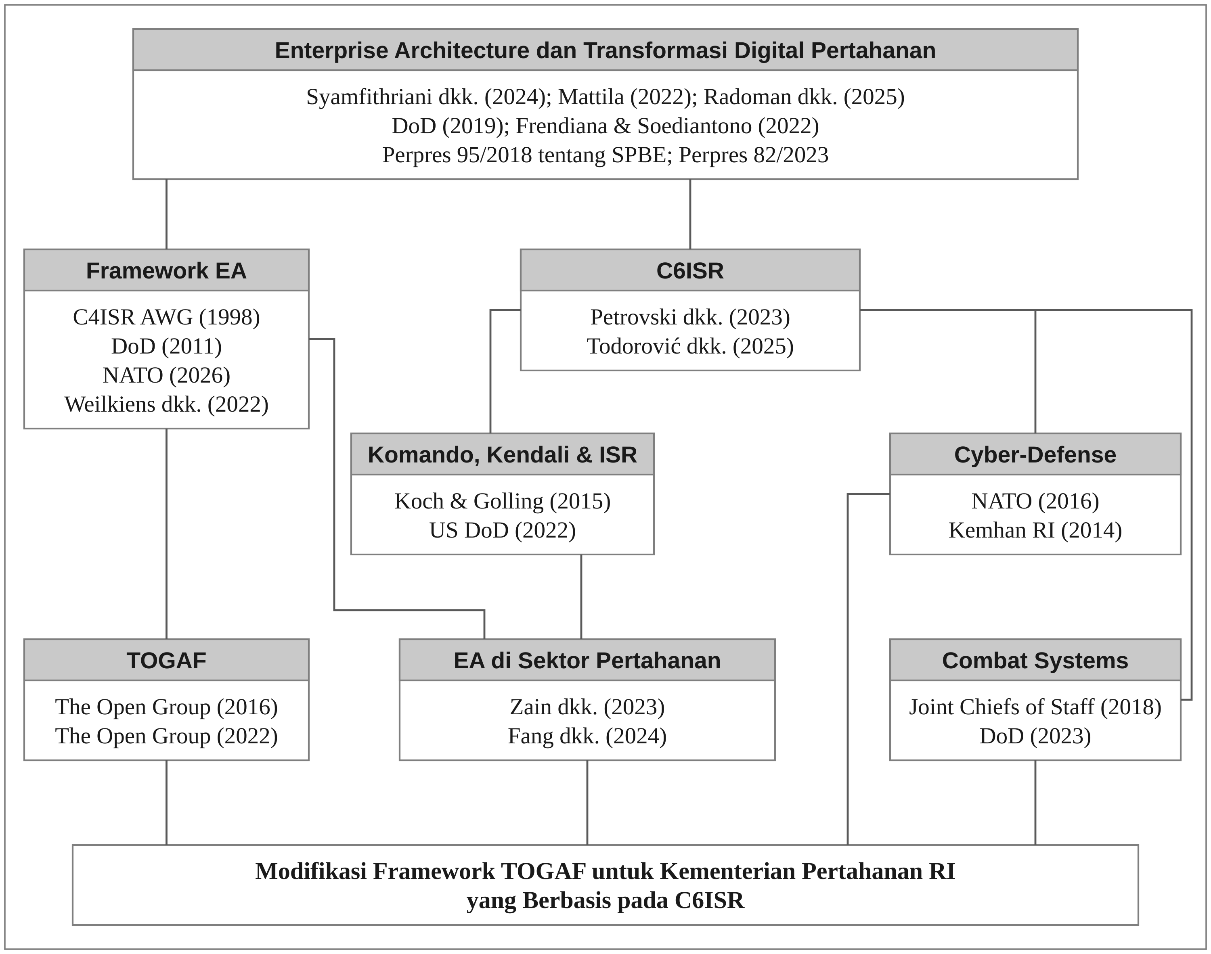
\includegraphics[width=1.00\linewidth,height=0.8\textheight,keepaspectratio]{images/Peta Literatur.png}
\caption{Peta Literatur}
\label{fig:II.1}
\end{figure}

Peta literatur tersebut terdiri atas dua cabang utama. Cabang pertama membahas \textit{framework} EA hingga TOGAF sebagai \textit{framework} yang dimodifikasi. Cabang kedua membahas C6ISR beserta unsur komando, kendali dan ISR, \textit{cyber-defense}, serta \textit{combat systems} sebagai dasar modifikasi. Penelitian EA di sektor pertahanan menjadi penghubung kedua cabang, dan seluruh cabang bermuara pada penelitian ini.

Tujuan peta literatur ini adalah menggali definisi dan informasi yang lebih mendalam terkait hal-hal yang diperlukan dalam penelitian ini. Hal-hal tersebut mencakup transformasi digital pertahanan, EA beserta \textit{framework}-nya, TOGAF, C6ISR, serta Kemhan RI sebagai objek penelitian.

\section{Transformasi Digital di Sektor Pertahanan}
\label{sec:II.2}

Subbab ini membahas konsep transformasi digital, praktiknya di sektor pertahanan, konsep pertahanan cerdas dan \textit{network centric warfare}, serta transformasi digital di Kemhan RI.

\subsection{Konsep Transformasi Digital}
\label{sec:II.2.1}

Transformasi digital adalah perubahan menyeluruh yang memanfaatkan teknologi digital untuk menciptakan nilai baru dan mengubah cara organisasi beroperasi. Transformasi digital berbeda dengan digitalisasi, karena tidak berhenti pada adopsi teknologi, tetapi juga mengubah proses bisnis, tata kelola, dan budaya organisasi.

\textcite{Bumann2019} mengidentifikasi enam bidang aksi transformasi digital, yaitu strategi, organisasi, budaya, teknologi, pelanggan, dan manusia, sebagaimana ditunjukkan pada Gambar~\ref{fig:II.2}. \textcite{Elia2024} melengkapi pandangan tersebut dengan menetapkan transformasi digital sebagai proses strategis yang menghubungkan kemampuan teknologi dengan kapabilitas organisasi, mulai dari tujuan, proses, mitra, manusia, dan platform, hingga perlindungan dan privasi data.
\begin{figure}[htbp]
\centering
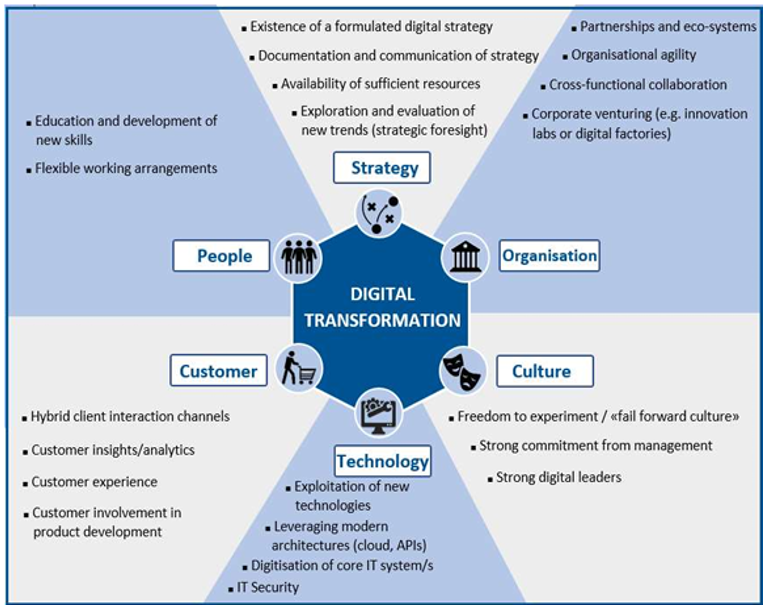
\includegraphics[width=0.79\linewidth,height=0.8\textheight,keepaspectratio]{images/DT_Verkuli.png}
\caption{Bidang Aksi Transformasi Digital}
\label{fig:II.2}
\end{figure}

Di Indonesia, RPJPN 2025–2045 menetapkan transformasi digital sebagai agenda pembangunan nasional untuk membangun ekosistem digital yang tangguh dan berdaulat. Ekosistem tersebut dibangun melalui penguatan infrastruktur digital, SDM digital, regulasi, integrasi data lintas sektor, serta riset dan inovasi \cite{UU59Tahun2024}.

\subsection{Praktik Transformasi Digital pertahanan}
\label{sec:II.2.2}

Transformasi digital menjadi kebutuhan di sektor pertahanan, termasuk industri pertahanan \cite{Frendiana2022}. Dibandingkan sektor publik pada umumnya, transformasi digital pertahanan lebih kompleks karena mencakup pengelolaan informasi strategis, interoperabilitas sistem senjata, keamanan siber, dan dukungan operasi militer secara \textit{real-time}. Praktik di beberapa negara menunjukkan bahwa transformasi digital pertahanan dijalankan sebagai strategi nasional, antara lain:
\begin{enumerate}[label=\arabic*.]
\item Amerika Serikat. \textit{DoD Digital Modernization Strategy} menetapkan empat prioritas, yaitu keamanan siber, kecerdasan buatan, \textit{cloud}, serta komando, kendali, dan komunikasi (C3). Prioritas tersebut dijabarkan ke dalam empat tujuan, yaitu inovasi untuk keunggulan kompetitif, optimalisasi efisiensi dan kapabilitas, penguatan keamanan siber untuk postur pertahanan yang tangguh, serta pengembangan talenta digital \cite{USDoD2019}, sebagaimana ditunjukkan pada Gambar~\ref{fig:II.3}.
\item Singapura. Strategi \textit{Total Defence} yang diperkenalkan sejak tahun 1984 memandang pertahanan sebagai tanggung jawab seluruh elemen bangsa. Pada tahun 2019, \textit{Digital Defence} ditambahkan sebagai pilar keenam untuk menghadapi ancaman dari ranah digital, melengkapi pilar \textit{Military}, \textit{Civil}, \textit{Economic}, \textit{Social}, dan \textit{Psychological Defence}. Pilar-pilar tersebut ditunjukkan pada Gambar~\ref{fig:II.4}.
\end{enumerate}
\begin{figure}[htbp]
\centering
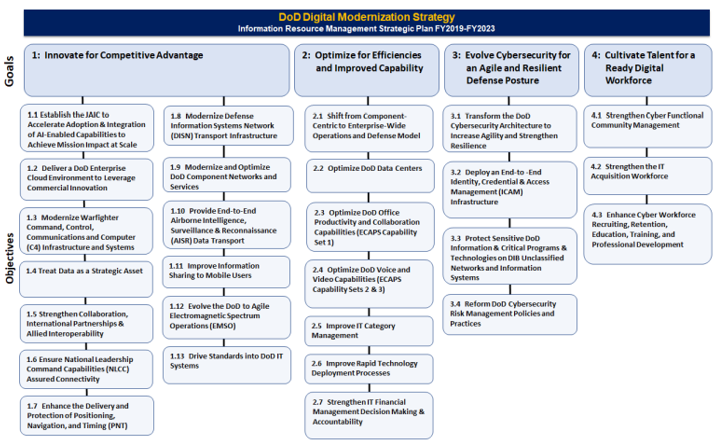
\includegraphics[width=1.00\linewidth,height=0.8\textheight,keepaspectratio]{images/DoD_Digital_Modernization_Strategy.png}
\caption{\textit{DoD Digital Modernization Strategy}}
\label{fig:II.3}
\end{figure}
\begin{figure}[htbp]
\centering
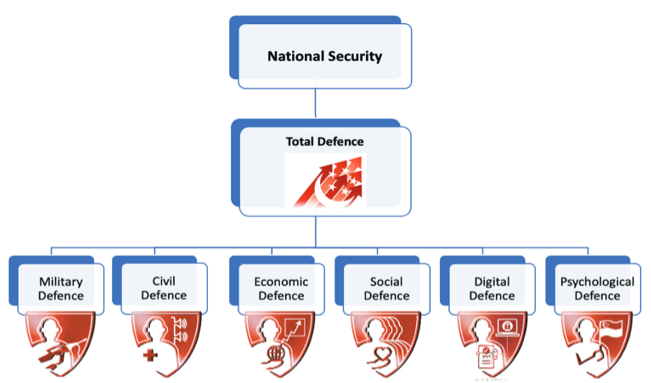
\includegraphics[width=0.79\linewidth,height=0.8\textheight,keepaspectratio]{images/Singapore_Total_Defence.png}
\caption{\textit{Total Defence} Singapura}
\label{fig:II.4}
\end{figure}

Kedua praktik tersebut menunjukkan bahwa transformasi digital pertahanan tidak hanya menyangkut teknologi, tetapi juga keamanan siber, talenta digital, dan keterlibatan lintas organisasi.

\subsection{Pertahanan Cerdas dan \textit{Network Centric Warfare}}
\label{sec:II.2.3}

Istilah \textit{smart defence} diperkenalkan NATO pada KTT Chicago 2012 sebagai pendekatan pengembangan kapabilitas melalui prioritisasi, spesialisasi, dan kerja sama multinasional \cite{NATO2012Forces2020}. Dalam penelitian ini, pertahanan cerdas dimaknai lebih luas sebagai pemanfaatan teknologi digital, data, dan sistem terintegrasi untuk meningkatkan efektivitas dan keunggulan pertahanan. Dalam paradigma ini, data diposisikan sebagai aset strategis, dan keunggulan informasi (\textit{information superiority}) menjadi penentu keunggulan operasi \cite{Koch2015}.

Konsep yang mendasari pertahanan cerdas adalah \textit{network centric warfare} (NCW). NCW menekankan bahwa kekuatan tempur berasal dari kemampuan menghubungkan sensor, komando dan kendali, unit tempur, dan pengambil keputusan dalam satu jaringan informasi, sehingga informasi dapat dibagikan secara \textit{real-time} \cite{Koch2015}. Gambar~\ref{fig:II.5} menunjukkan arsitektur NCW yang terdiri atas lapisan darat, udara, dan antariksa. Setiap simpul dapat bertukar data melalui beberapa jalur alternatif, sehingga jaringan tetap berfungsi meskipun sebagian simpul terganggu.
\begin{figure}[htbp]
\centering
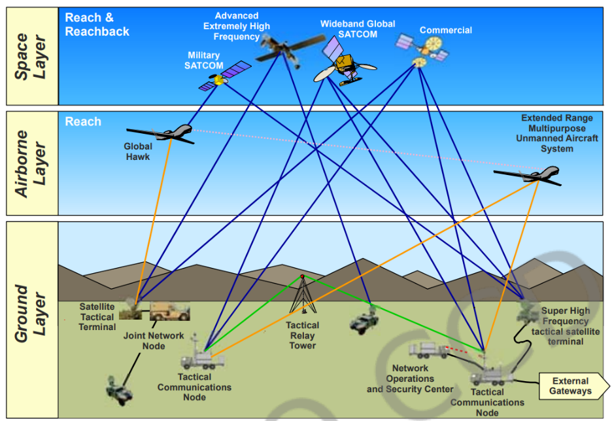
\includegraphics[width=0.93\linewidth,height=0.8\textheight,keepaspectratio]{images/Arsitektur_NCW.png}
\caption{Arsitektur \textit{Network Centric Warfare}}
\label{fig:II.5}
\end{figure}

NCW kemudian berkembang menjadi \textit{Joint All-Domain Command and Control} (JADC2), yaitu strategi Departemen Pertahanan Amerika Serikat untuk mengintegrasikan komando dan kendali lintas domain darat, laut, udara, antariksa, dan siber \cite{USDoD2022}. JADC2 dibangun atas tiga fungsi, yaitu \textit{sense} (mengumpulkan dan membagikan data dari seluruh domain), \textit{make sense} (mengolah data menjadi pemahaman situasi), dan \textit{act} (mengambil serta mendistribusikan keputusan secara cepat dan aman), sebagaimana ditunjukkan pada Gambar~\ref{fig:II.6}.
\begin{figure}[htbp]
\centering
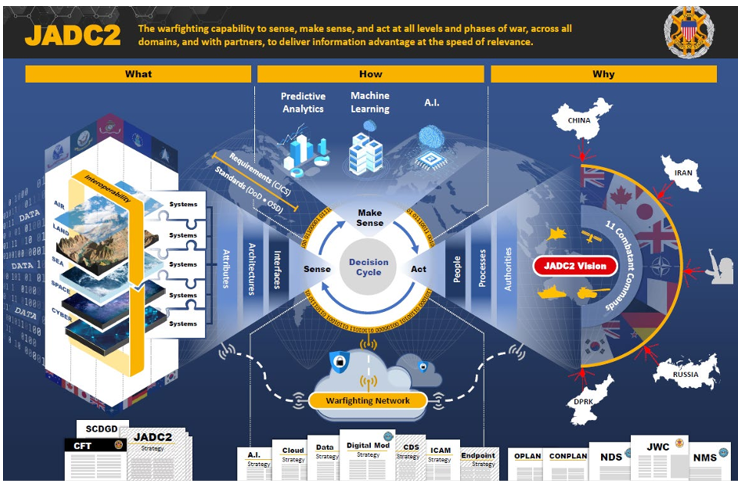
\includegraphics[width=1.00\linewidth,height=0.8\textheight,keepaspectratio]{images/Arsitektur_JADC2.png}
\caption{Strategi \textit{Joint All-Domain Command and Control} (JADC2)}
\label{fig:II.6}
\end{figure}

NCW dan JADC2 menunjukkan bahwa keunggulan pertahanan modern bergantung pada integrasi data, interoperabilitas, dan keamanan jaringan.

\subsection{Transformasi Digital Kemhan RI}
\label{sec:II.2.4}

Transformasi digital Kemhan RI merupakan bagian dari modernisasi pertahanan sekaligus pembenahan tata kelola pemerintahan. Sebagai kementerian, Kemhan RI terikat pada kebijakan pemerintah digital nasional. Sebagai institusi pertahanan, Kemhan RI juga dituntut mendukung keterpaduan komando dan kendali lintas matra TNI.

Landasan kebijakan nasional transformasi digital Kemhan RI adalah sebagai berikut:
\begin{enumerate}[label=\arabic*.]
\item Sistem Pemerintahan Berbasis Elektronik (SPBE). Perpres Nomor 95 Tahun 2018 mewajibkan setiap instansi pusat menyusun Arsitektur SPBE dan Peta Rencana SPBE untuk jangka waktu lima tahun \cite{Perpres95Tahun2018}, dengan berpedoman pada Arsitektur SPBE Nasional \cite{Perpres132Tahun2022}.
\item Percepatan transformasi digital. Perpres Nomor 82 Tahun 2023 mendorong keterpaduan layanan digital nasional, antara lain melalui aplikasi SPBE prioritas yang digunakan bersama oleh instansi pemerintah \cite{Perpres82Tahun2023}. Upaya tersebut diperkuat dengan pembentukan Komite Percepatan Transformasi Digital Pemerintah yang mengoordinasikan dan menyinkronkan transformasi digital lintas instansi \cite{Perpres83Tahun2025}.
\item Tata kelola data. Kebijakan Satu Data Indonesia dijabarkan di sektor pertahanan melalui Permenhan Nomor 1 Tahun 2023 tentang Satu Data Pertahanan. Peraturan tersebut menetapkan penyelenggara Satu Data Pertahanan, yaitu pengarah, walidata, produsen data, pengolah data, pengaman sistem data, dan forum Satu Data Pertahanan, serta Portal Satu Data Pertahanan sebagai media bagi pakai data \cite{Permenhan1Tahun2023}.
\end{enumerate}

Di lingkungan pertahanan, arah transformasi digital juga ditentukan oleh kebijakan keamanan siber dan kelembagaan. Pedoman Pertahanan Siber menjadi acuan dalam menghadapi ancaman terhadap perangkat keras, perangkat lunak, serta data dan informasi pertahanan \cite{Permenhan82Tahun2014}. Pelindungan infrastruktur informasi vital sektor pertahanan juga telah memiliki peta jalan untuk tahun 2025–2029 \cite{Permenhan34Tahun2025}. Secara kelembagaan, pengelolaan data, sistem informasi, dan infrastruktur TIK merupakan tugas Pusat Data dan Informasi (Pusdatin) \cite{Permenhan30Tahun2025}, yang juga berperan sebagai Walidata Satu Data Pertahanan \cite{Pusdatin2026SatuData}.

Pelaksanaan kebijakan tersebut telah menunjukkan sejumlah capaian. Indeks SPBE Kemhan RI meningkat dari 2,62 pada tahun 2022 menjadi 3,43 pada tahun 2023 dengan predikat Baik, dengan peningkatan utama pada indikator kebijakan internal manajemen data \cite{Pusdatin2024}. Pada tata kelola data, Indeks Satu Data Indonesia Kemhan RI tahun 2025 mencapai 81,35, di atas rata-rata nasional tahun 2024 sebesar 51,07 \cite{Pusdatin2026SatuData}. Kemhan RI juga mulai mengintegrasikan layanan digitalnya, antara lain melalui penerapan \textit{Single Sign-On} (SSO) yang menghubungkan berbagai aplikasi satuan kerja melalui satu identitas pengguna \cite{Pusdatin2026SSO}.

Meskipun demikian, capaian tersebut masih bersifat parsial. Evaluasi Satu Data Pertahanan tahun 2026 menunjukkan bahwa Indeks Pembangunan Statistik Kemhan RI tahun 2024 masih berpredikat Cukup dengan nilai 2,14, sedangkan pengelolaan informasi geospasial tahun 2025 baru berada pada tingkat Operasional dengan nilai 2,54. Evaluasi tersebut juga mengidentifikasi empat kendala utama, yaitu kelembagaan dan koordinasi, kualitas data, integrasi sistem, serta kapasitas SDM \cite{Pusdatin2026SatuData}. Tantangan transformasi digital Kemhan RI selengkapnya dirangkum per dimensi pada Tabel~\ref{tab:II.1}.
\begingroup\small\setstretch{1.0}
\begin{longtable}{@{}>{\raggedright\arraybackslash}p{0.065\linewidth}>{\raggedright\arraybackslash}p{0.162\linewidth}>{\raggedright\arraybackslash}p{0.389\linewidth}>{\raggedright\arraybackslash}p{0.291\linewidth}@{}}
\caption{Tantangan Transformasi Digital Kemhan RI}\label{tab:II.1}\\
\toprule
\textbf{No.} & \textbf{Dimensi} & \textbf{Kondisi Saat Ini} & \textbf{Dampak}\\
\midrule
\endfirsthead
\multicolumn{4}{@{}l}{\small\itshape \tablename\ \thetable{} (lanjutan)}\\
\toprule
\textbf{No.} & \textbf{Dimensi} & \textbf{Kondisi Saat Ini} & \textbf{Dampak}\\
\midrule
\endhead
\bottomrule
\endlastfoot
\centering\arraybackslash 1 & Tata kelola & Pusdatin berperan menjalankan sistem yang sudah ada, dan belum ada fungsi yang mengorkestrasi transformasi lintas satuan kerja dan matra. Kelembagaan dan koordinasi menjadi kendala utama. & Perencanaan dan pengembangan sistem berjalan sendiri-sendiri per satuan kerja.\\
\centering\arraybackslash 2 & Data & Data terkotak per aplikasi. Kamus data, klasifikasi data, dan kanal berbagi pakai belum tersedia, serta kualitas data dan statistik sektoral belum optimal. & Data sulit dibagi pakai dan dianalisis lintas domain.\\
\centering\arraybackslash 3 & Aplikasi & Terdapat 247 aplikasi (176 umum dan 71 khusus). Sebagian aplikasi khusus memiliki fungsi serupa dan mekanisme autentikasi yang berbeda. & Investasi berulang dan integrasi antaraplikasi sulit dilakukan.\\
\centering\arraybackslash 4 & Teknologi & Seluruh layanan bertumpu pada satu \textit{data center} tanpa \textit{disaster recovery center}. & Terdapat titik tunggal kegagalan (\textit{single point of failure}).\\
\centering\arraybackslash 5 & Keamanan siber & Pengamanan masih parsial, sedangkan konektivitas yang makin tinggi memperbesar dampak intrusi. & Layanan dan data pertahanan rentan terhadap gangguan dan serangan siber.\\
\centering\arraybackslash 6 & SDM & Kompetensi digital, statistik, dan geospasial belum merata. & Kualitas implementasi bergantung pada kemampuan masing-masing unit.\\
\centering\arraybackslash 7 & Operasional & Komando dan kendali dikembangkan per matra, dan sistem dengan standar berbeda sulit bertukar informasi. & Keterpaduan ISR, komando-kendali, dan unsur penindak dalam operasi gabungan sulit dicapai.\\
\end{longtable}
\endgroup

Tabel~\ref{tab:II.1} menunjukkan bahwa tantangan transformasi digital Kemhan RI saling terkait dan mencakup seluruh lapisan organisasi, mulai dari tata kelola hingga operasional. Oleh karena itu, transformasi digital Kemhan RI tidak dapat dilakukan secara parsial per aplikasi atau per satuan kerja, tetapi membutuhkan acuan menyeluruh yang menautkan strategi dengan proses bisnis, data, aplikasi, teknologi, dan kapabilitas operasional.

\section{\textit{Enterprise Architecture} (EA)}
\label{sec:II.3}

Istilah \textit{Enterprise Architecture} (EA) tersusun atas dua konsep, yaitu \textit{enterprise} dan arsitektur. TOGAF memandang \textit{enterprise} sebagai kumpulan organisasi yang memiliki tujuan bersama, sehingga \textit{enterprise} dapat berupa satu kementerian beserta seluruh satuan kerjanya. Adapun arsitektur adalah konsep atau sifat fundamental suatu sistem yang diwujudkan dalam elemen-elemennya, hubungan antarelemen, serta prinsip perancangan dan evolusinya \cite{TOGAF2022}.

Lankhorst mendefinisikan EA sebagai satu kesatuan prinsip, metode, dan model yang koheren, yang digunakan dalam perancangan dan perwujudan struktur organisasi, proses bisnis, sistem informasi, dan infrastruktur suatu \textit{enterprise} \cite{Lankhorst2017}. Ross dkk. memandang EA sebagai logika pengorganisasian (\textit{organizing logic}) proses bisnis dan infrastruktur TI yang mencerminkan kebutuhan integrasi dan standardisasi model operasi organisasi \cite{Ross2006}. Kedua definisi tersebut menunjukkan bahwa EA tidak hanya menyangkut teknologi, tetapi juga keterpaduan seluruh komponen organisasi.

EA mendeskripsikan kondisi saat ini (\textit{baseline} atau \textit{as-is}), kondisi yang diinginkan (\textit{target} atau \textit{to-be}), serta peta jalan (\textit{roadmap}) untuk berpindah dari kondisi saat ini menuju kondisi target \cite{Tamm2011}. Deskripsi tersebut disusun dalam beberapa domain arsitektur. TOGAF membagi EA ke dalam empat domain utama, yaitu bisnis, data, aplikasi, dan teknologi, serta memungkinkan penambahan domain lain sesuai kebutuhan, misalnya keamanan \cite{TOGAF2022}. Hubungan antardomain dan antarkondisi tersebut ditunjukkan pada Gambar~\ref{fig:II.7}.
\begin{figure}[htbp]
\centering
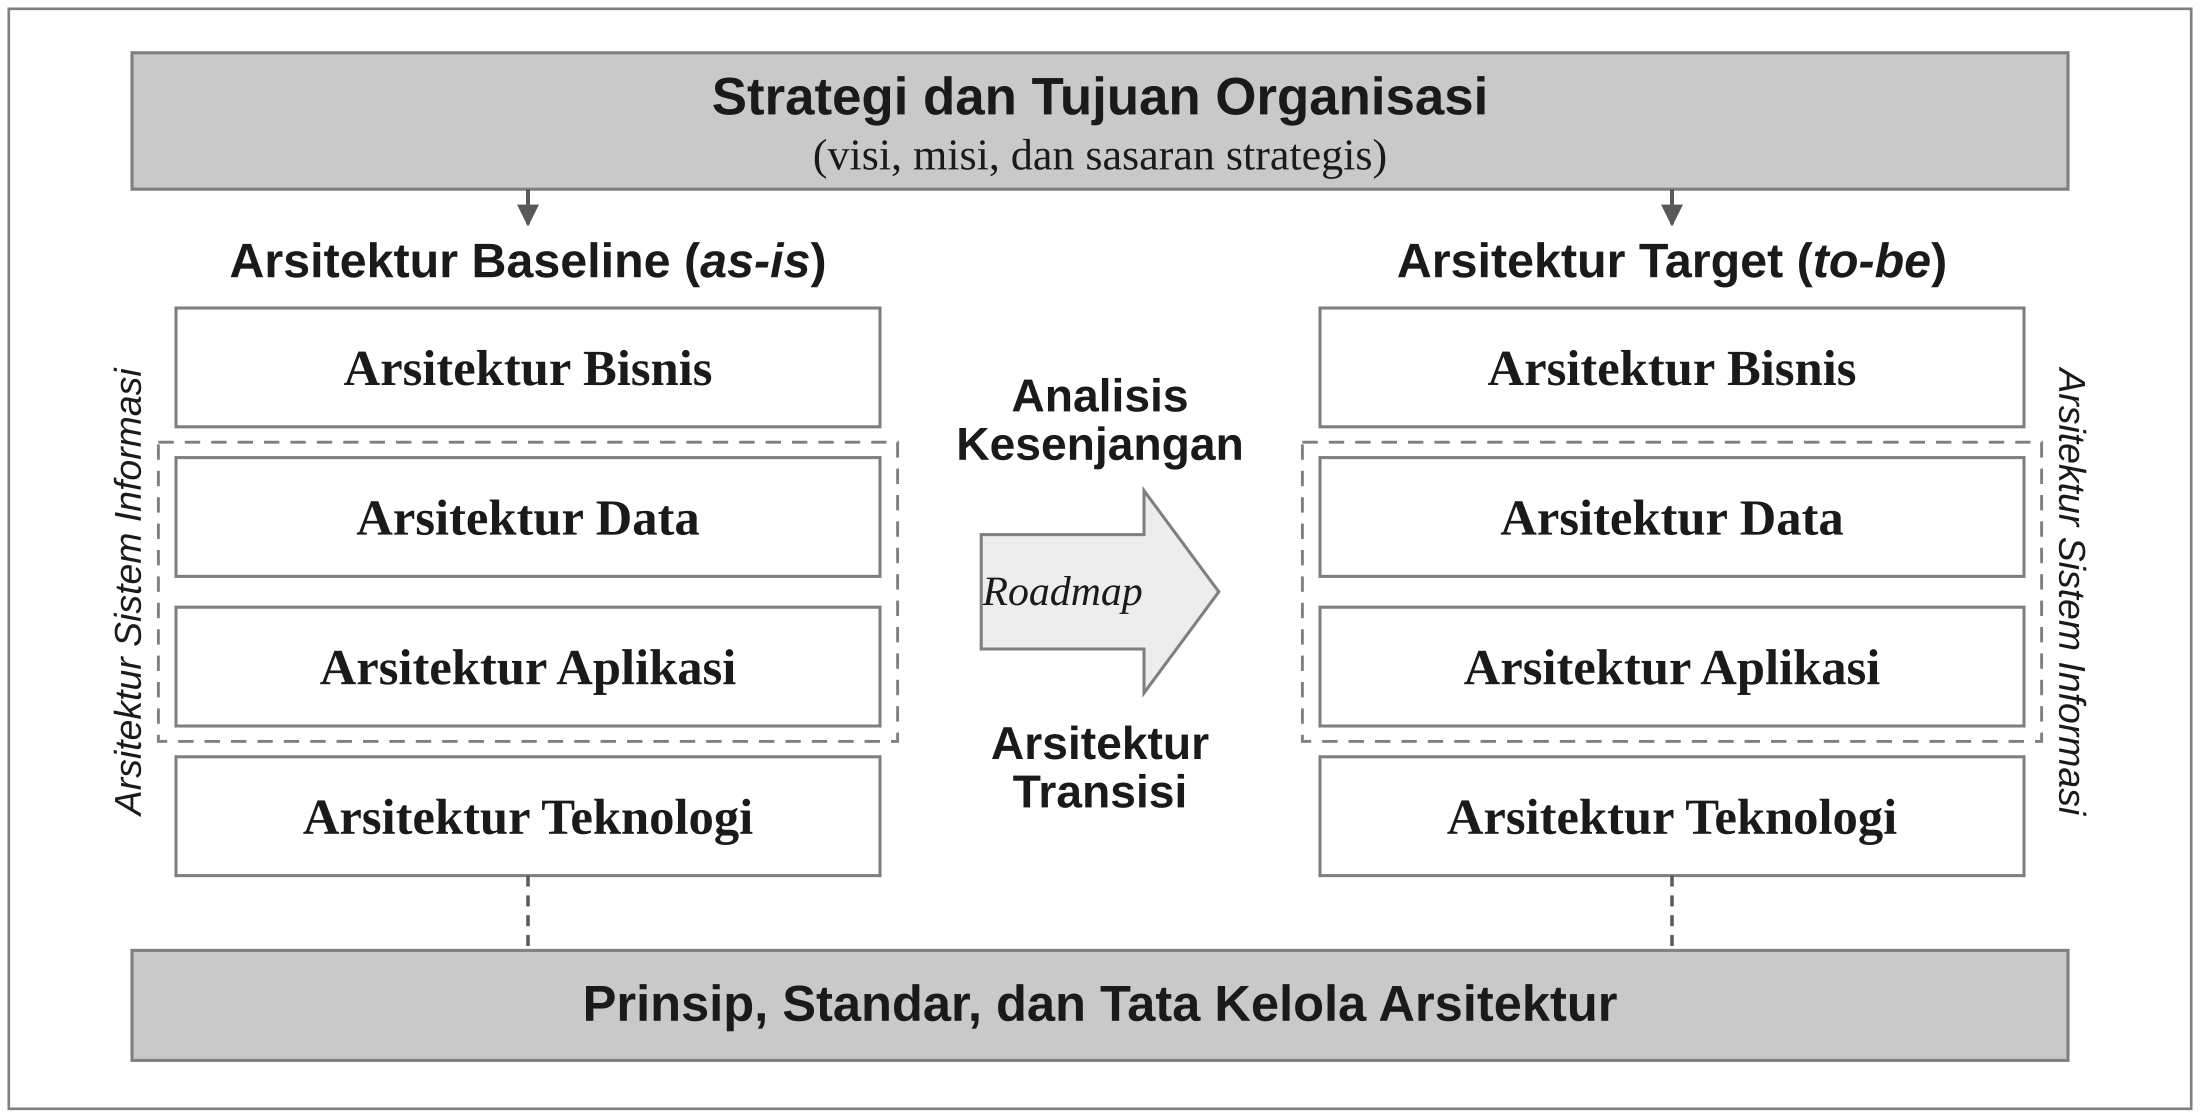
\includegraphics[width=1.00\linewidth,height=0.8\textheight,keepaspectratio]{images/Domain dan Kondisi Arsitektur EA.png}
\caption{Domain dan Kondisi Arsitektur dalam EA}
\label{fig:II.7}
\end{figure}

Gambar~\ref{fig:II.7} menunjukkan bahwa strategi dan tujuan organisasi menjadi titik awal yang mengarahkan seluruh domain arsitektur. Arsitektur bisnis mendeskripsikan strategi, tata kelola, organisasi, dan proses bisnis. Arsitektur data mendeskripsikan struktur aset data dan pengelolaannya. Arsitektur aplikasi mendeskripsikan aplikasi yang mendukung proses bisnis beserta interaksinya. Arsitektur teknologi mendeskripsikan perangkat keras, perangkat lunak, dan jaringan yang menopang ketiga domain lainnya \cite{TOGAF2022}. Arsitektur data dan arsitektur aplikasi secara bersama-sama disebut arsitektur sistem informasi. Setiap domain dirancang pada kondisi \textit{baseline} dan \textit{target}, kemudian kesenjangan di antara keduanya menjadi dasar penyusunan \textit{roadmap} dan arsitektur transisi. Konsistensi seluruh rancangan dijaga oleh prinsip, standar, dan tata kelola arsitektur.

Dalam penelitian ini, EA dimaknai sebagai rancangan menyeluruh yang menyelaraskan strategi Kemhan RI dengan proses bisnis, data, aplikasi, teknologi, dan kapabilitas operasional pertahanan, beserta \textit{roadmap} untuk mewujudkannya. Pemaknaan ini sejalan dengan keterbukaan TOGAF terhadap penambahan domain arsitektur, yang menjadi dasar penambahan domain C6ISR dalam penelitian ini.

\subsection{Manfaat EA dalam Transformasi Digital}
\label{sec:II.3.1}

Transformasi digital menuntut perubahan serentak pada strategi, proses bisnis, data, dan teknologi. Tanpa acuan bersama, perubahan tersebut berisiko berjalan sendiri-sendiri dan justru menambah kompleksitas. Kajian literatur sistematis oleh Syamfithriani dkk. menunjukkan bahwa EA berperan penting dalam mendukung transformasi digital, terutama dalam merancang dan mengelola infrastruktur TI untuk menekan risiko dan kompleksitas, sehingga transformasi berjalan efisien dan efektif \cite{Syamfithriani2024}.

Tamm dkk. menjelaskan bahwa EA memberikan nilai bagi organisasi melalui empat manfaat (\textit{benefit enablers}) \cite{Tamm2011}. Keempatnya relevan dengan tantangan Kemhan RI pada Tabel~\ref{tab:II.1}, yaitu sebagai berikut:
\begin{enumerate}[label=\arabic*.]
\item Keselarasan organisasi (\textit{organisational alignment}), yaitu keselarasan antara strategi organisasi dan teknologi informasi (TI).
\item Ketersediaan informasi (\textit{information availability}), yaitu tersedianya informasi yang berkualitas dan konsisten bagi pengambil keputusan.
\item Optimalisasi portofolio sumber daya (\textit{resource portfolio optimisation}), yaitu pengelolaan portofolio aplikasi dan infrastruktur secara efisien, termasuk mengurangi duplikasi.
\item Komplementaritas sumber daya (\textit{resource complementarity}), yaitu kemampuan berbagai sumber daya TI untuk saling melengkapi dan bekerja bersama.
\end{enumerate}

Selain memberikan manfaat, EA juga memandang transformasi sebagai proses bertahap. Ross dkk. mengidentifikasi empat tahap kematangan arsitektur yang dilalui organisasi, yaitu \textit{business silos}, \textit{standardized technology}, \textit{optimized core}, dan \textit{business modularity} \cite{Ross2006}, sebagaimana ditunjukkan pada Gambar~\ref{fig:II.8}.
\begin{figure}[htbp]
\centering
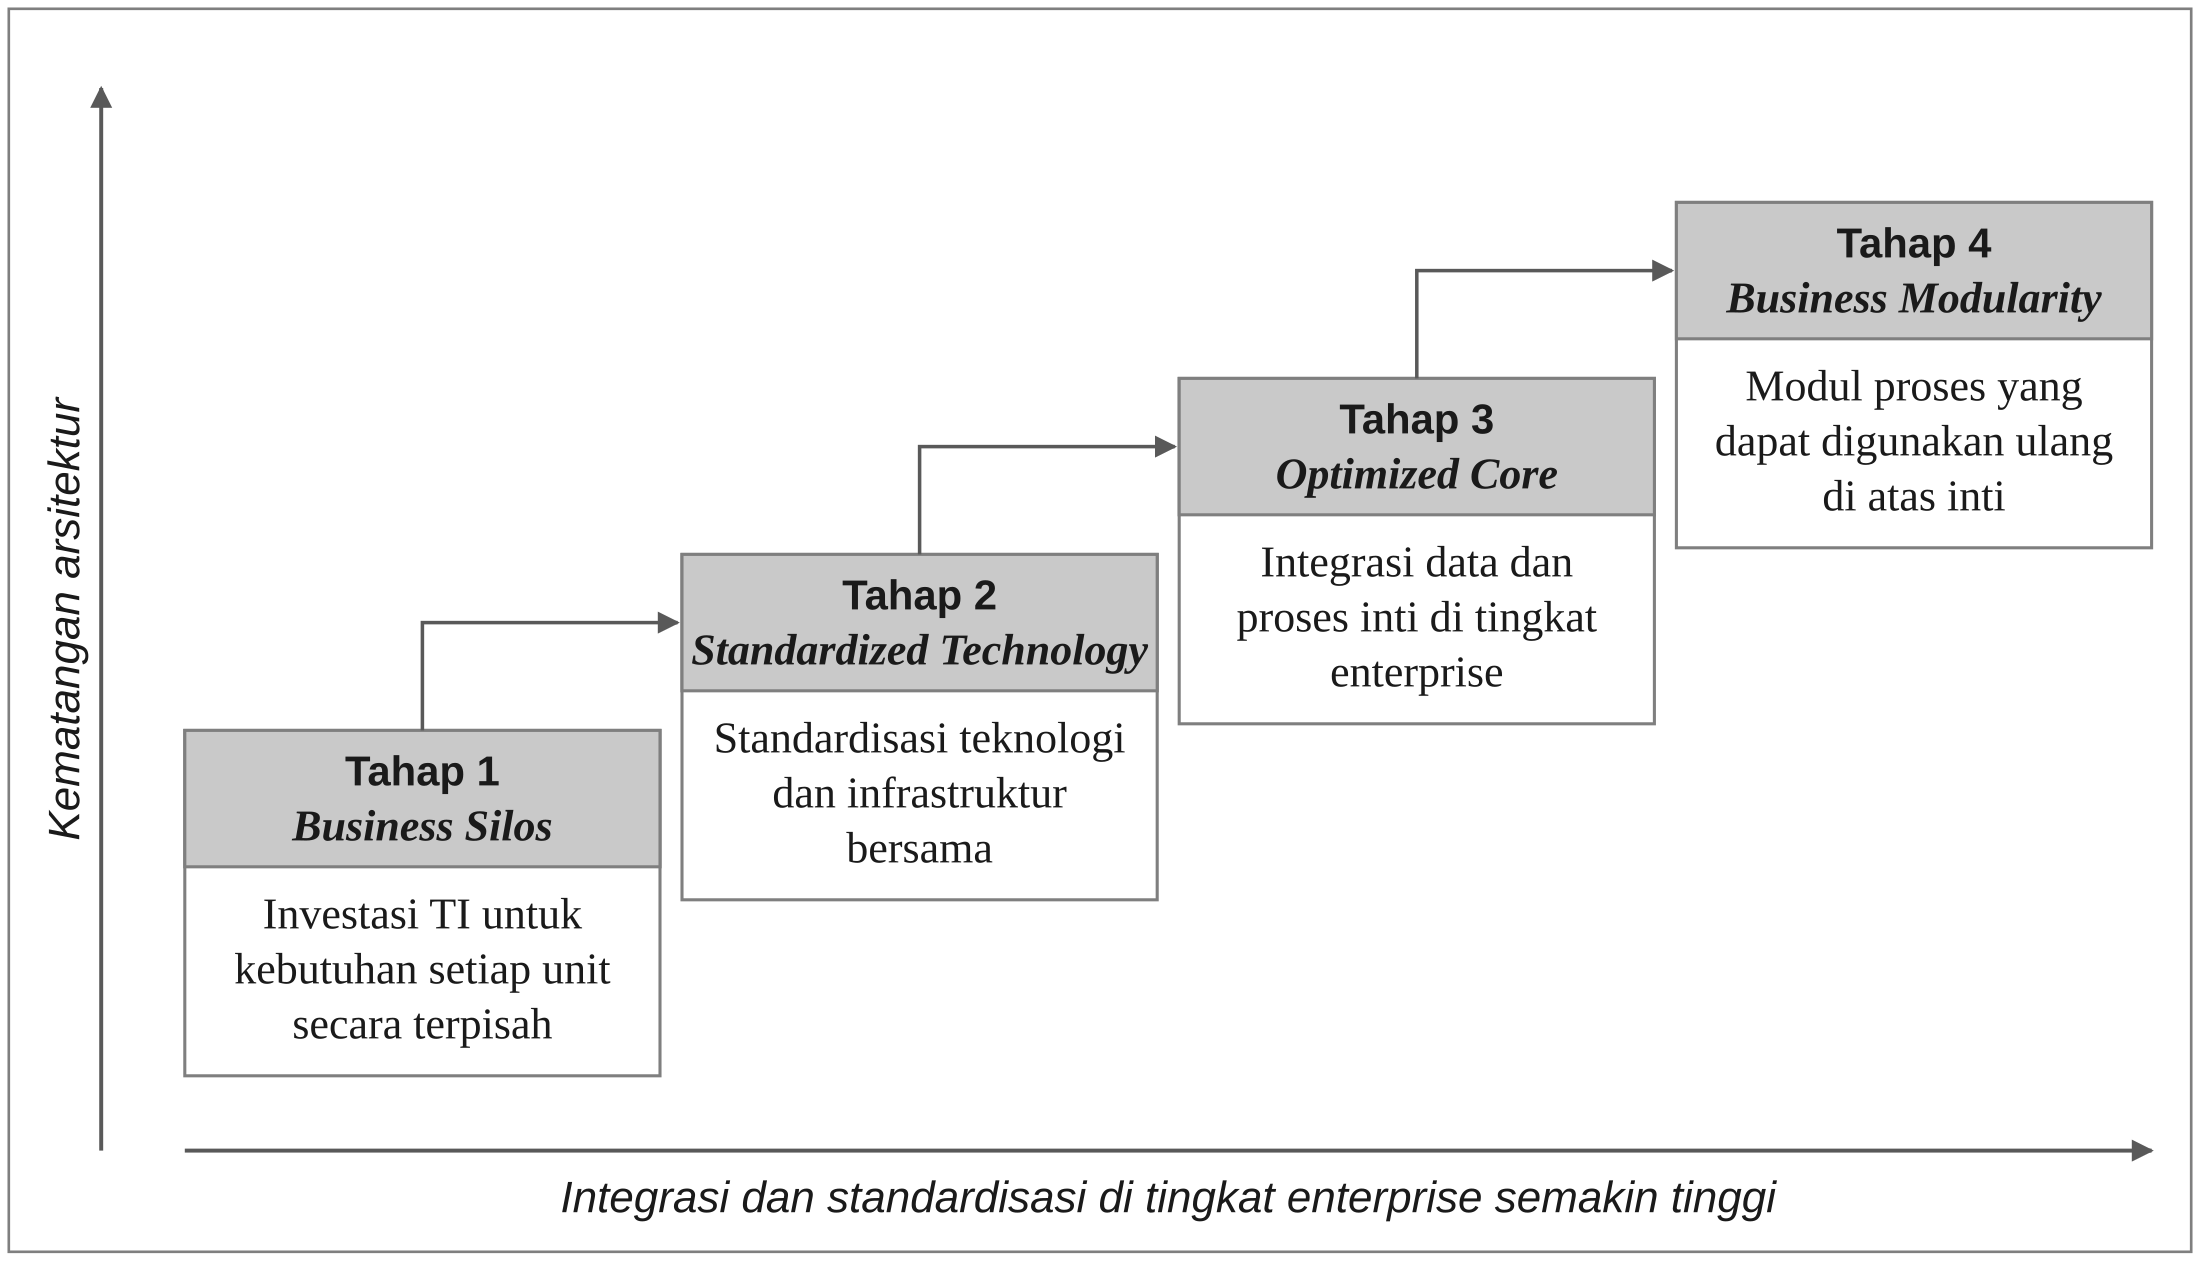
\includegraphics[width=1.00\linewidth,height=0.8\textheight,keepaspectratio]{images/Tahap Kematangan Arsitektur Ross.png}
\caption{Tahap Kematangan Arsitektur Menurut Ross dkk.}
\label{fig:II.8}
\end{figure}

Pada tahap \textit{business silos}, investasi TI ditujukan untuk memenuhi kebutuhan setiap unit secara terpisah. Tahap \textit{standardized technology} menstandarkan teknologi dan infrastruktur bersama untuk meningkatkan efisiensi. Tahap \textit{optimized core} mengintegrasikan data dan proses inti di tingkat \textit{enterprise}, sedangkan tahap \textit{business modularity} menyusun modul proses yang dapat digunakan ulang di atas inti tersebut untuk meningkatkan ketangkasan organisasi \cite{Ross2006}.

Pada organisasi militer, Mattila menemukan bahwa metode tata kelola TIK yang umum belum diterapkan secara optimal dan belum menjawab seluruh permasalahan transformasi militer \cite{Mattila2022}. Temuan tersebut menunjukkan bahwa EA beserta \textit{framework} pendukungnya perlu disesuaikan dengan karakteristik organisasi pertahanan.

\subsection{Arsitektur SPBE sebagai EA Pemerintah Indonesia}
\label{sec:II.3.2}

Di Indonesia, penerapan EA pada instansi pemerintah diwujudkan melalui Arsitektur SPBE. Perpres Nomor 95 Tahun 2018 mendefinisikan Arsitektur SPBE sebagai kerangka dasar yang mendeskripsikan integrasi proses bisnis, data dan informasi, infrastruktur SPBE, aplikasi SPBE, dan keamanan SPBE untuk menghasilkan layanan SPBE yang terintegrasi. Arsitektur SPBE terdiri atas Arsitektur SPBE Nasional, Arsitektur SPBE Instansi Pusat, dan Arsitektur SPBE Pemerintah Daerah \cite{Perpres95Tahun2018}.

Arsitektur SPBE Instansi Pusat disusun dengan berpedoman pada Arsitektur SPBE Nasional dan rencana strategis instansi. Arsitektur tersebut berlaku untuk jangka waktu lima tahun, ditetapkan oleh pimpinan instansi, dan direviu pada paruh waktu dan tahun terakhir pelaksanaan atau sewaktu-waktu sesuai kebutuhan \cite{Perpres95Tahun2018}. Arsitektur SPBE Nasional ditetapkan melalui Perpres Nomor 132 Tahun 2022 dan memuat arah kebijakan dan strategi, kerangka kerja, referensi arsitektur, domain arsitektur, serta inisiatif strategis. Referensi arsitektur berisi komponen dasar arsitektur yang baku sebagai acuan, sedangkan domain arsitektur berisi substansi arsitektur. Keduanya mencakup enam domain, yaitu proses bisnis, data dan informasi, layanan, aplikasi, infrastruktur, dan keamanan \cite{Perpres132Tahun2022}. Keenam domain tersebut memiliki padanan dengan domain TOGAF sebagaimana ditunjukkan pada Tabel~\ref{tab:II.2}.
\begingroup\small\setstretch{1.0}
\begin{longtable}{@{}>{\raggedright\arraybackslash}p{0.241\linewidth}>{\raggedright\arraybackslash}p{0.415\linewidth}>{\raggedright\arraybackslash}p{0.281\linewidth}@{}}
\caption{Pemetaan Domain Arsitektur SPBE dan Domain TOGAF}\label{tab:II.2}\\
\toprule
\textbf{Domain Arsitektur SPBE} & \textbf{Cakupan} & \textbf{Padanan pada TOGAF}\\
\midrule
\endfirsthead
\multicolumn{3}{@{}l}{\small\itshape \tablename\ \thetable{} (lanjutan)}\\
\toprule
\textbf{Domain Arsitektur SPBE} & \textbf{Cakupan} & \textbf{Padanan pada TOGAF}\\
\midrule
\endhead
\bottomrule
\endlastfoot
Proses Bisnis & Fungsi dan proses penyelenggaraan pemerintahan & \textit{Business Architecture}\\
Layanan & Layanan administrasi pemerintahan dan layanan publik berbasis elektronik & \textit{Business Architecture} (layanan bisnis)\\
Data dan Informasi & Data dan informasi yang digunakan dan dihasilkan oleh proses bisnis & \textit{Data Architecture}\\
Aplikasi & Aplikasi yang mendukung proses bisnis dan layanan & \textit{Application Architecture}\\
Infrastruktur & Pusat data, jaringan intra, dan sistem penghubung layanan & \textit{Technology Architecture}\\
Keamanan & Pengamanan data, aplikasi, dan infrastruktur & \textit{Security Architecture} (lintas domain)\\
\end{longtable}
\endgroup

Tabel~\ref{tab:II.2} menunjukkan bahwa domain Arsitektur SPBE selaras dengan domain TOGAF. Perbedaannya, keamanan ditetapkan sebagai domain tersendiri dalam Arsitektur SPBE, sedangkan TOGAF memperlakukannya sebagai \textit{concern} lintas domain \cite{TOGAFRiskSecurity}. Selain itu, Arsitektur SPBE lebih menekankan muatan dan referensi arsitektur yang harus dipenuhi, sedangkan langkah pengembangannya dapat menggunakan metode dari \textit{framework} EA, seperti TOGAF ADM. Dengan demikian, TOGAF dapat digunakan untuk menyusun arsitektur yang memenuhi kewajiban Arsitektur SPBE.

\section{\textit{Framework} EA Pertahanan}
\label{sec:II.4}

\textit{Framework} EA menyediakan struktur, sudut pandang (\textit{viewpoint}), dan panduan untuk mendeskripsikan serta mengembangkan arsitektur. Di lingkungan pertahanan, \textit{framework} EA yang banyak digunakan adalah DoDAF, NAF, dan MODAF \cite{Weilkiens2022}. Ketiganya berakar pada \textit{C4ISR Architecture Framework}, yaitu kerangka yang dikembangkan Departemen Pertahanan Amerika Serikat untuk menyeragamkan deskripsi arsitektur sistem komando, kendali, komunikasi, komputer, intelijen, pengawasan, dan pengintaian \cite{C4ISRAWG1998}. Perkembangan ketiga \textit{framework} tersebut ditunjukkan pada Gambar~\ref{fig:II.9}.
\begin{figure}[htbp]
\centering
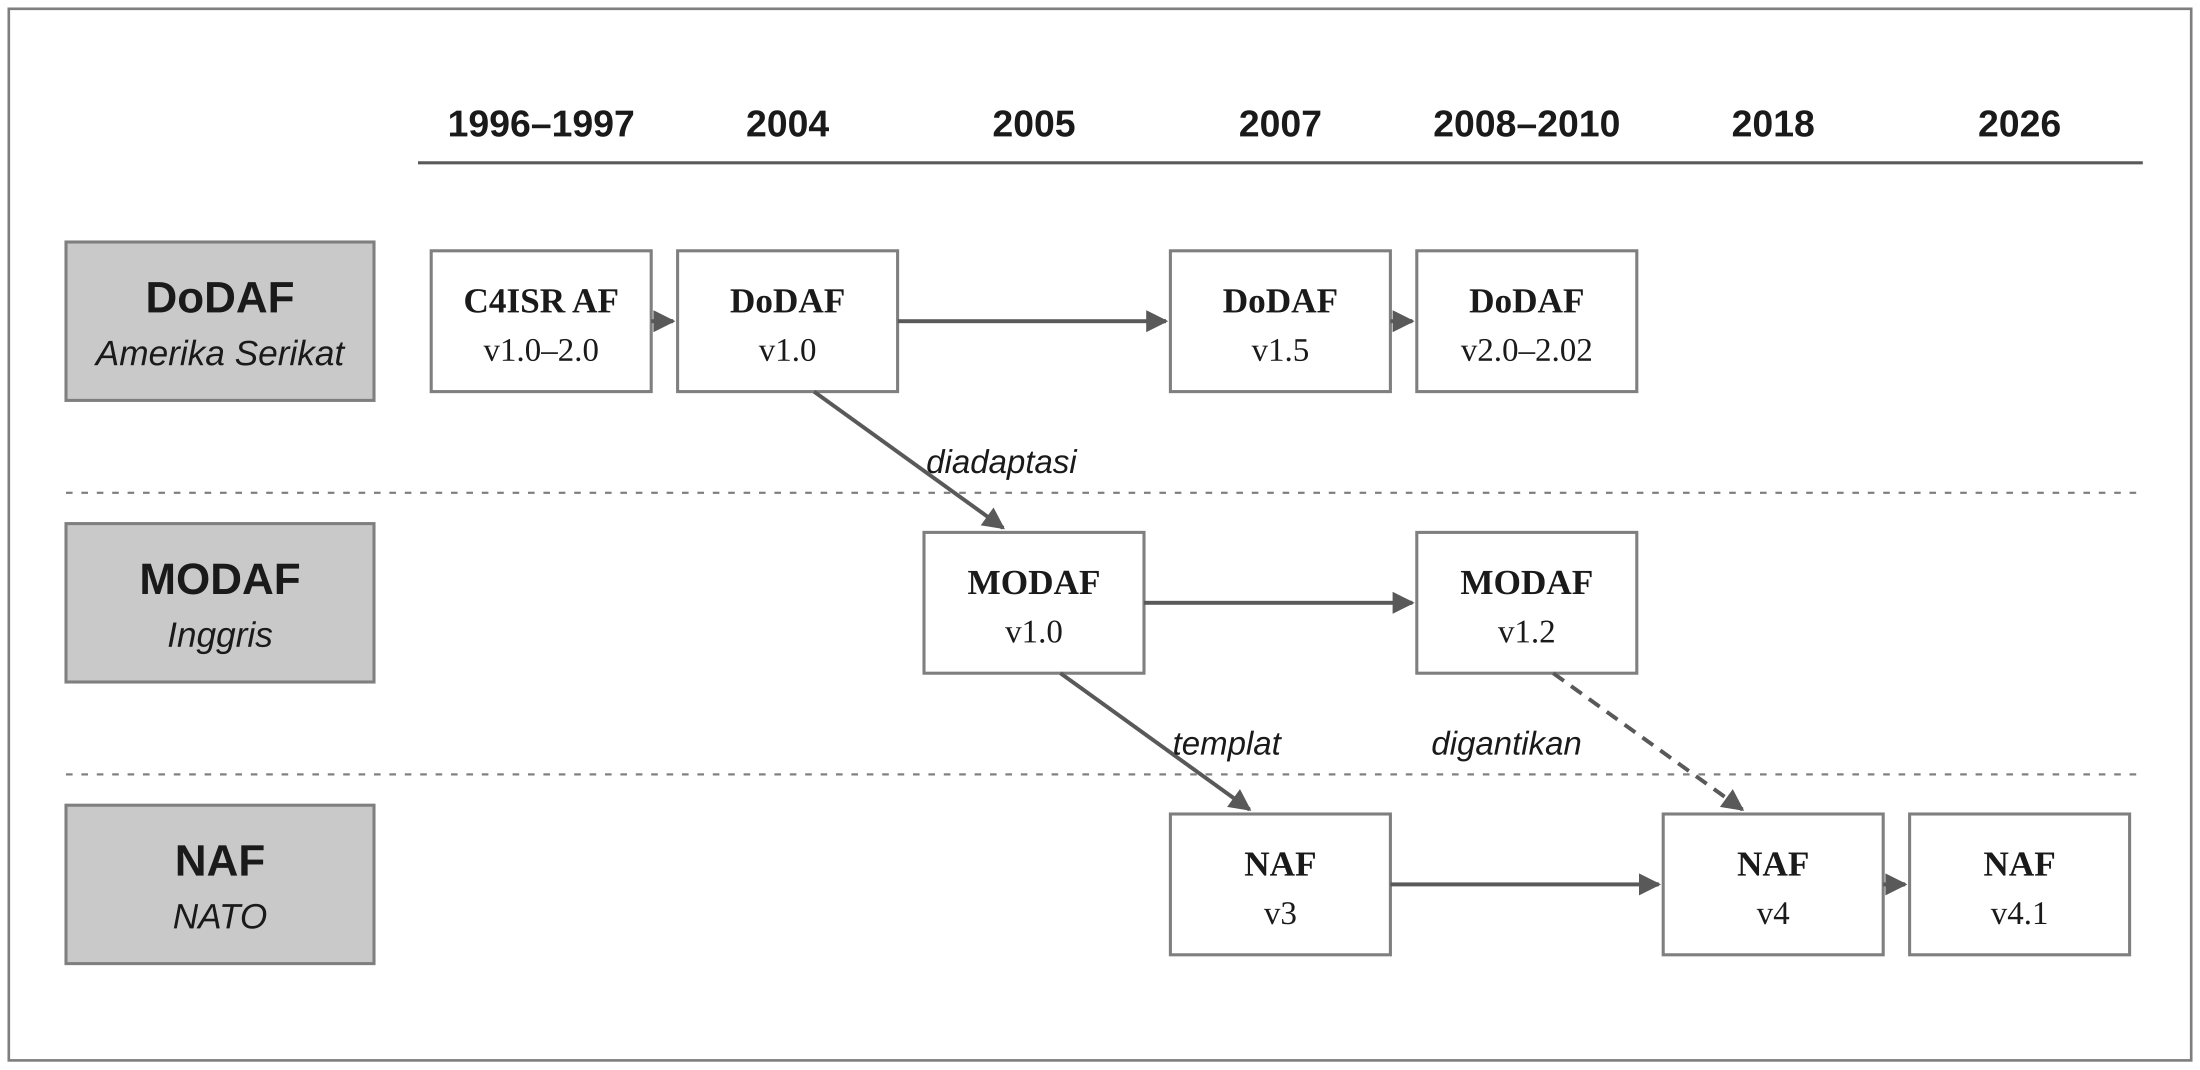
\includegraphics[width=1.00\linewidth,height=0.8\textheight,keepaspectratio]{images/Perkembangan Framework EA Pertahanan.png}
\caption{Perkembangan \textit{Framework} EA Pertahanan}
\label{fig:II.9}
\end{figure}

Gambar~\ref{fig:II.9} menunjukkan bahwa DoDAF berkembang langsung dari \textit{C4ISR Architecture Framework}. MODAF diadaptasi dari DoDAF versi 1.0 dan kemudian menjadi acuan bagi NAF versi 3. Selanjutnya, MODAF digantikan oleh NAF versi 4 \cite{MODAF2012}. Karena memiliki akar yang sama, ketiga \textit{framework} tersebut kuat dalam merepresentasikan kapabilitas, operasi, dan interoperabilitas sistem militer.

\subsection{DoDAF}
\label{sec:II.4.1}

\textit{Department of Defense Architecture Framework} (DoDAF) dikembangkan Departemen Pertahanan Amerika Serikat untuk membantu pengambil keputusan melalui pengorganisasian dan berbagi informasi lintas departemen, komponen, dan program \cite{DoDAF2010v202}. DoDAF berevolusi dari \textit{C4ISR Architecture Framework}, kemudian berkembang menjadi DoDAF versi 1.0 (2004), 1.5 (2007), 2.0 (2009), hingga versi 2.02 sebagai versi yang berlaku saat ini. Perubahan terpenting terjadi pada versi 2.0, yaitu pergeseran dari pendekatan berbasis produk menjadi berbasis data melalui \textit{DoDAF Meta Model} (DM2), sehingga model arsitektur dapat dipilih sesuai tujuan penggunaannya (\textit{fit-for-purpose}) \cite{DoDAF2010v202}.

DoDAF 2.02 mengelompokkan 52 model ke dalam delapan \textit{viewpoint}, sebagaimana ditunjukkan pada Gambar~\ref{fig:II.10} \cite{DoDAF2010v202}.
\begin{figure}[htbp]
\centering
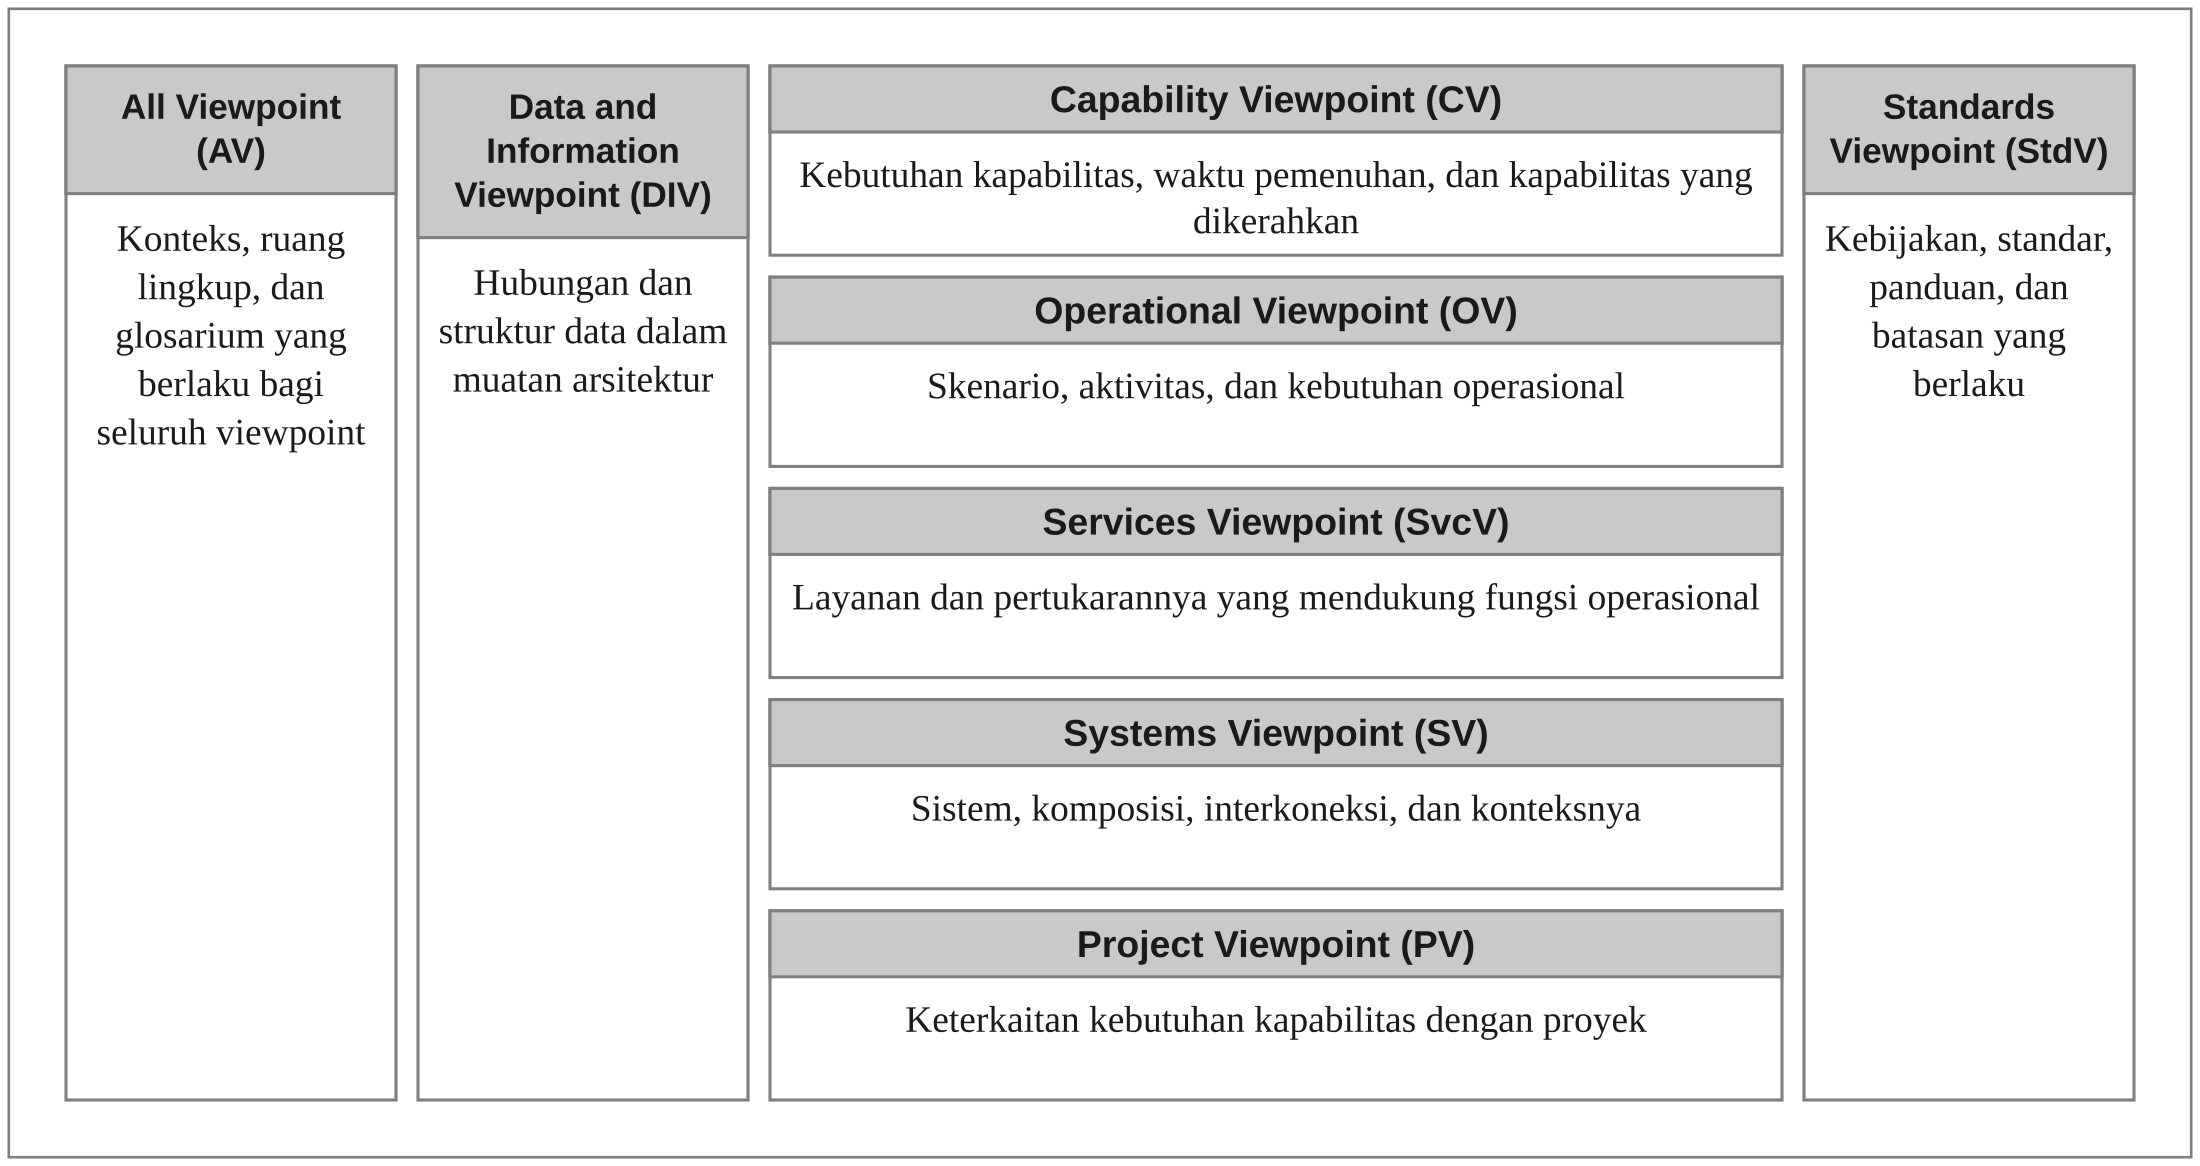
\includegraphics[width=1.00\linewidth,height=0.8\textheight,keepaspectratio]{images/Viewpoint DoDAF 2.02.png}
\caption{\textit{Viewpoint} DoDAF 2.02}
\label{fig:II.10}
\end{figure}

Gambar~\ref{fig:II.10} menunjukkan bahwa \textit{All Viewpoint}, \textit{Data and Information Viewpoint}, dan \textit{Standards Viewpoint} berlaku bagi seluruh model, sedangkan \textit{Capability}, \textit{Operational}, \textit{Services}, \textit{Systems}, dan \textit{Project Viewpoint} menggambarkan arsitektur mulai dari kebutuhan kapabilitas hingga implementasinya. Untuk menyusun model tersebut, DoDAF menyediakan enam langkah pengembangan arsitektur, yaitu menentukan tujuan penggunaan, menentukan ruang lingkup, menentukan data yang dibutuhkan, mengumpulkan dan mengorganisasi data, melakukan analisis, serta mendokumentasikan hasil \cite{DoDAF2010v202}.

Langkah tersebut masih bersifat umum, sedangkan sebagian besar muatan DoDAF berupa ketentuan tentang apa yang harus dideskripsikan. Selain itu, DoDAF dirancang untuk mendukung proses inti Departemen Pertahanan Amerika Serikat, seperti pengembangan kapabilitas gabungan, perencanaan dan penganggaran, serta akuisisi pertahanan \cite{DoDAF2010v202}. Oleh karena itu, penerapan DoDAF di luar lingkungan tersebut memerlukan penyesuaian.

\subsection{NAF}
\label{sec:II.4.2}

\textit{NATO Architecture Framework} (NAF) dikembangkan NATO sebagai standar untuk mengembangkan dan mendeskripsikan arsitektur, baik untuk kebutuhan militer maupun bisnis. NAF versi 4 (NAFv4) diterbitkan pada Januari 2018, sedangkan versi terbarunya, NAFv4.1, diterbitkan pada Maret 2026 oleh \textit{Architecture Capability Team} di bawah \textit{Digital Policy Committee} \cite{NAFv41}. NAFv4 terdiri atas tiga komponen utama, yaitu metodologi untuk mengembangkan arsitektur dan menjalankan proyek arsitektur, \textit{viewpoint} sebagai konvensi penyusunan \textit{view} arsitektur, serta meta-model yang memanfaatkan meta-model komersial, seperti ArchiMate dan UAF. NAFv4 juga diselaraskan dengan model konseptual ISO/IEC/IEEE 42010 \cite{NAFv41}.

Ciri khas NAFv4 adalah penyusunan \textit{viewpoint} dalam bentuk \textit{grid} dua dimensi, sebagaimana ditunjukkan pada Gambar~\ref{fig:II.11}. Baris \textit{grid} menunjukkan subjek perhatian (\textit{subjects of concern}), yaitu \textit{Concepts} (C), \textit{Service Specifications} (S), \textit{Logical Specifications} (L), \textit{Physical Resource Specifications} (P), dan \textit{Architecture Foundation} (A). Kolom \textit{grid} menunjukkan aspek perhatian (\textit{aspects of concern}), yaitu taksonomi, struktur, konektivitas, perilaku yang terdiri atas proses, status, dan urutan, serta informasi, batasan, dan \textit{roadmap} \cite{NAFv41,Lundberg2026}. Setiap sel merupakan satu \textit{viewpoint}, misalnya C1 \textit{Capability Taxonomy} dan Cr \textit{Capability Roadmap} \cite{NAFv41}.
\begin{figure}[htbp]
\centering
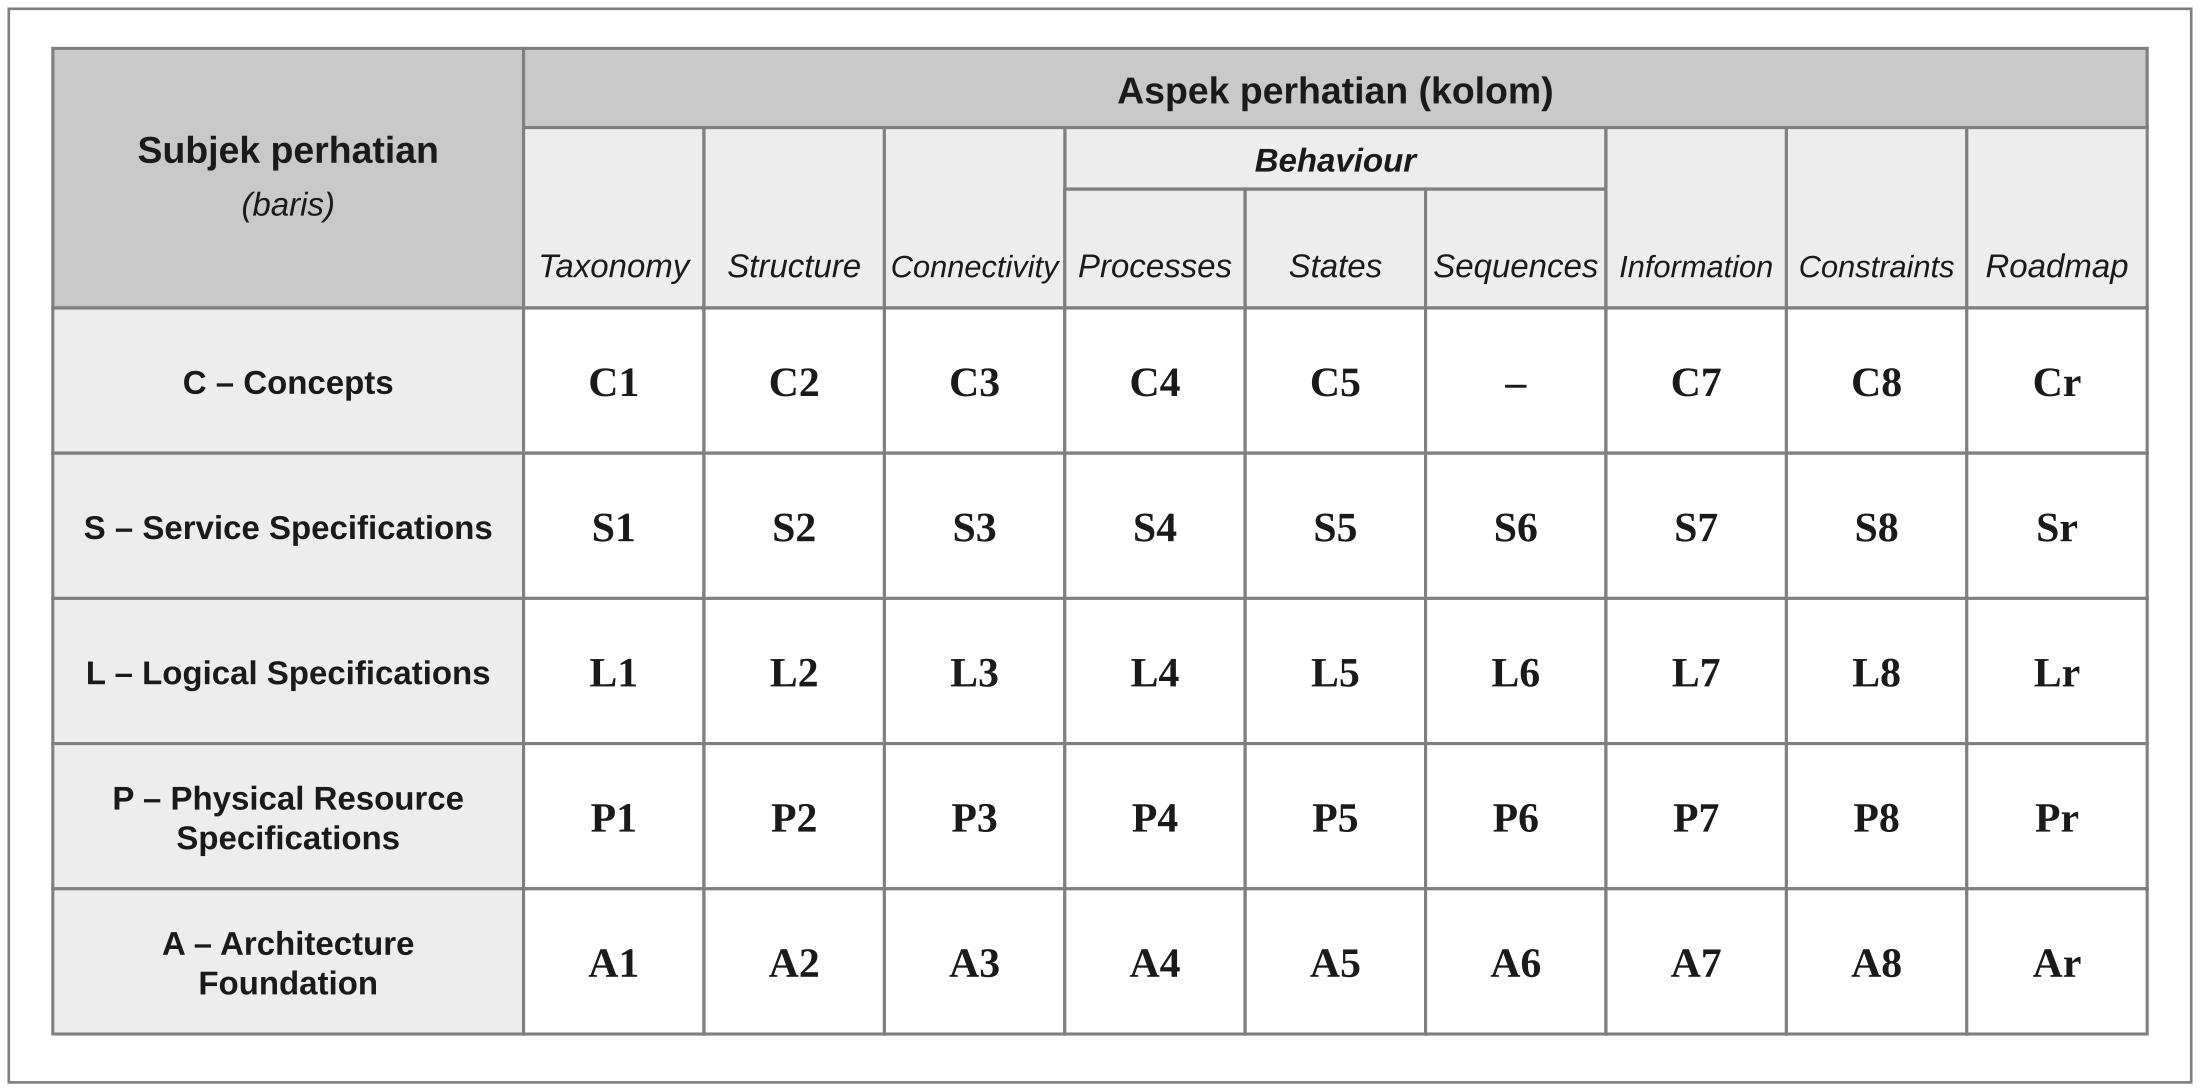
\includegraphics[width=1.00\linewidth,height=0.8\textheight,keepaspectratio]{images/Grid Viewpoint NAF v4.1.png}
\caption{\textit{Grid Viewpoint} NAFv4.1}
\label{fig:II.11}
\end{figure}

Berbeda dengan DoDAF, NAFv4 dilengkapi metodologi pengembangan arsitektur. Metodologi tersebut terdiri atas delapan tahap yang diterapkan pada tingkat \textit{enterprise} maupun proyek, yaitu \textit{establish architecture landscape}, \textit{establish architecture vision}, \textit{describe alternatives of architectures}, \textit{evaluate alternatives of architectures and propose trade-off}, \textit{develop migration plan}, \textit{govern application of architectures}, \textit{decide on architecture changes}, serta \textit{manage architecture motivation data and dashboard} \cite{NAFv41}.

Meskipun demikian, NAF dirancang untuk mendukung interoperabilitas multinasional di lingkungan NATO dan mengikuti kebijakan NATO \cite{NAFv41}. Oleh karena itu, penerapan NAF di Indonesia, yang bukan anggota NATO, memerlukan penyesuaian terhadap kebijakan nasional.

\subsection{MODAF}
\label{sec:II.4.3}

\textit{Ministry of Defence Architecture Framework} (MODAF) dikembangkan Kementerian Pertahanan Inggris untuk mendukung perencanaan pertahanan dan manajemen perubahan. MODAF diadaptasi dari DoDAF versi 1.0, kemudian diperluas dan disesuaikan dengan kebutuhan Kementerian Pertahanan Inggris \cite{MODAF2012}. Versi pertamanya dirilis pada tahun 2005. Dibandingkan DoDAF versi 1.0, MODAF menambahkan \textit{Strategic Views} dan \textit{Acquisition Views} untuk mendukung pengelolaan kapabilitas dan program pengadaan \cite{Weilkiens2022}. Secara keseluruhan, MODAF memiliki tujuh \textit{viewpoint}, sebagaimana ditunjukkan pada Gambar~\ref{fig:II.12} \cite{MODAF2012}.
\begin{figure}[htbp]
\centering
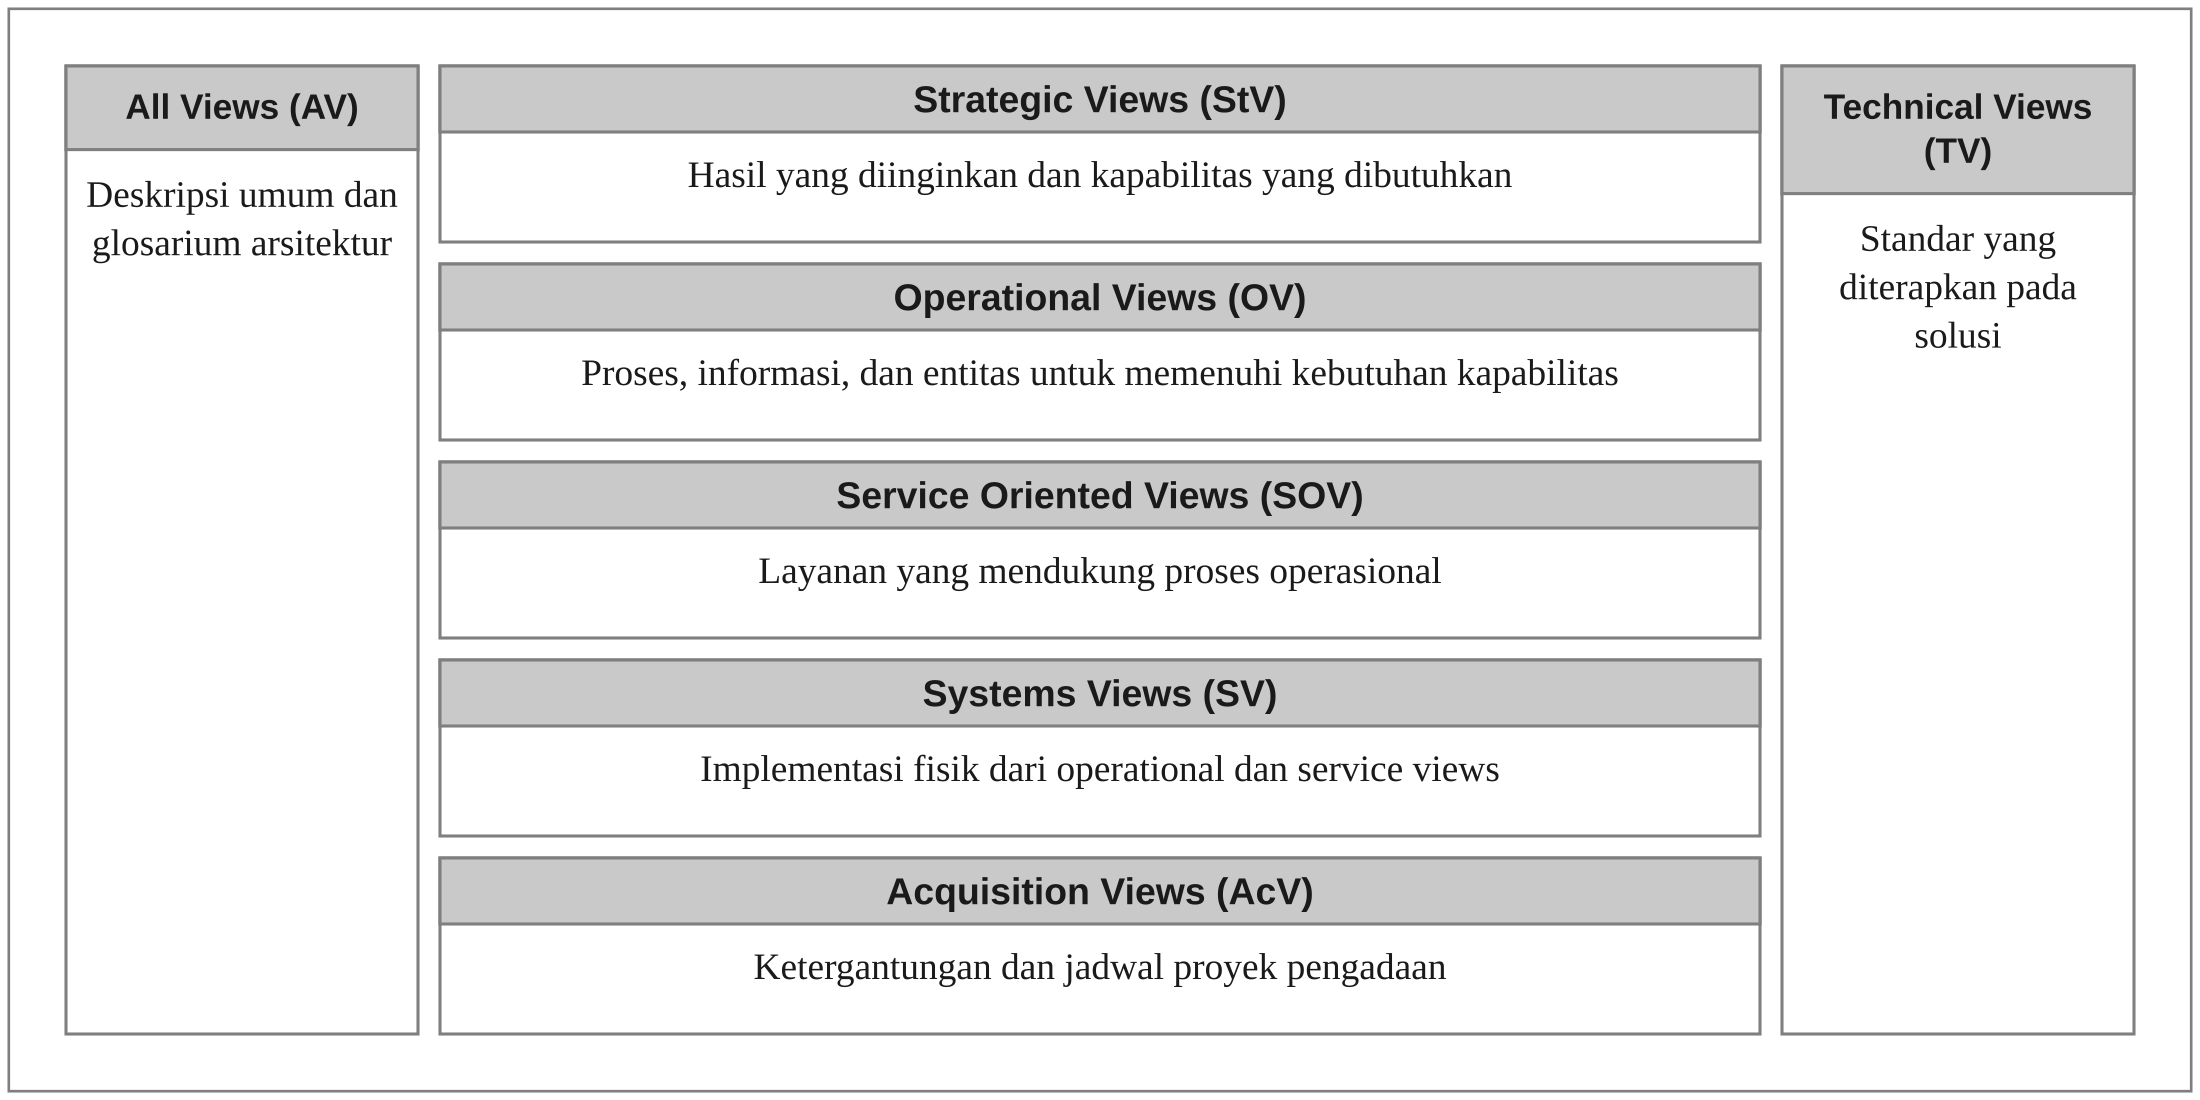
\includegraphics[width=1.00\linewidth,height=0.8\textheight,keepaspectratio]{images/Viewpoint MODAF.png}
\caption{\textit{Viewpoint} MODAF}
\label{fig:II.12}
\end{figure}

Gambar~\ref{fig:II.12} menunjukkan bahwa \textit{Strategic Views} menjadi titik awal yang menetapkan hasil yang diinginkan dan kapabilitas yang dibutuhkan. Kapabilitas tersebut kemudian dijabarkan ke dalam \textit{Operational}, \textit{Service Oriented}, dan \textit{Systems Views}. \textit{Acquisition Views} menggambarkan ketergantungan dan jadwal proyek pengadaan, sedangkan \textit{Technical Views} dan \textit{All Views} memuat standar serta deskripsi umum arsitektur \cite{MODAF2012}. MODAF kini telah digantikan oleh NAFv4 \cite{MODAF2012}, sehingga dalam penelitian ini MODAF menjadi rujukan bagi konsep \textit{viewpoint} strategis dan akuisisi.

\section{TOGAF}
\label{sec:II.5}

\textit{The Open Group Architecture Framework} (TOGAF) merupakan standar EA yang dikembangkan oleh The Open Group dan menyediakan kerangka, serta metode bersama bagi praktik EA. Versi pertamanya diterbitkan pada tahun 1995 dengan dasar \textit{Technical Architecture Framework for Information Management} (TAFIM) milik Departemen Pertahanan Amerika Serikat, sedangkan versi terkininya adalah \textit{TOGAF Standard, 10th Edition} yang dirilis pada tahun 2022. TOGAF digunakan oleh organisasi komersial, instansi pemerintah, organisasi publik nonpemerintah, hingga lembaga pertahanan \cite{TOGAF2022}.

\subsection{Struktur dan Komponen TOGAF}
\label{sec:II.5.1}

TOGAF 10 dirancang dengan memisahkan konsep yang bersifat universal dari konfigurasi yang bersifat rinci. Oleh karena itu, TOGAF dibagi menjadi dua bagian, yaitu \textit{TOGAF Fundamental Content} yang memuat konsep dan praktik inti, serta \textit{TOGAF Series Guides} yang memberikan panduan konfigurasi untuk kebutuhan tertentu \cite{TOGAF2022}. Struktur tersebut ditunjukkan pada Gambar~\ref{fig:II.13}.
\begin{figure}[htbp]
\centering
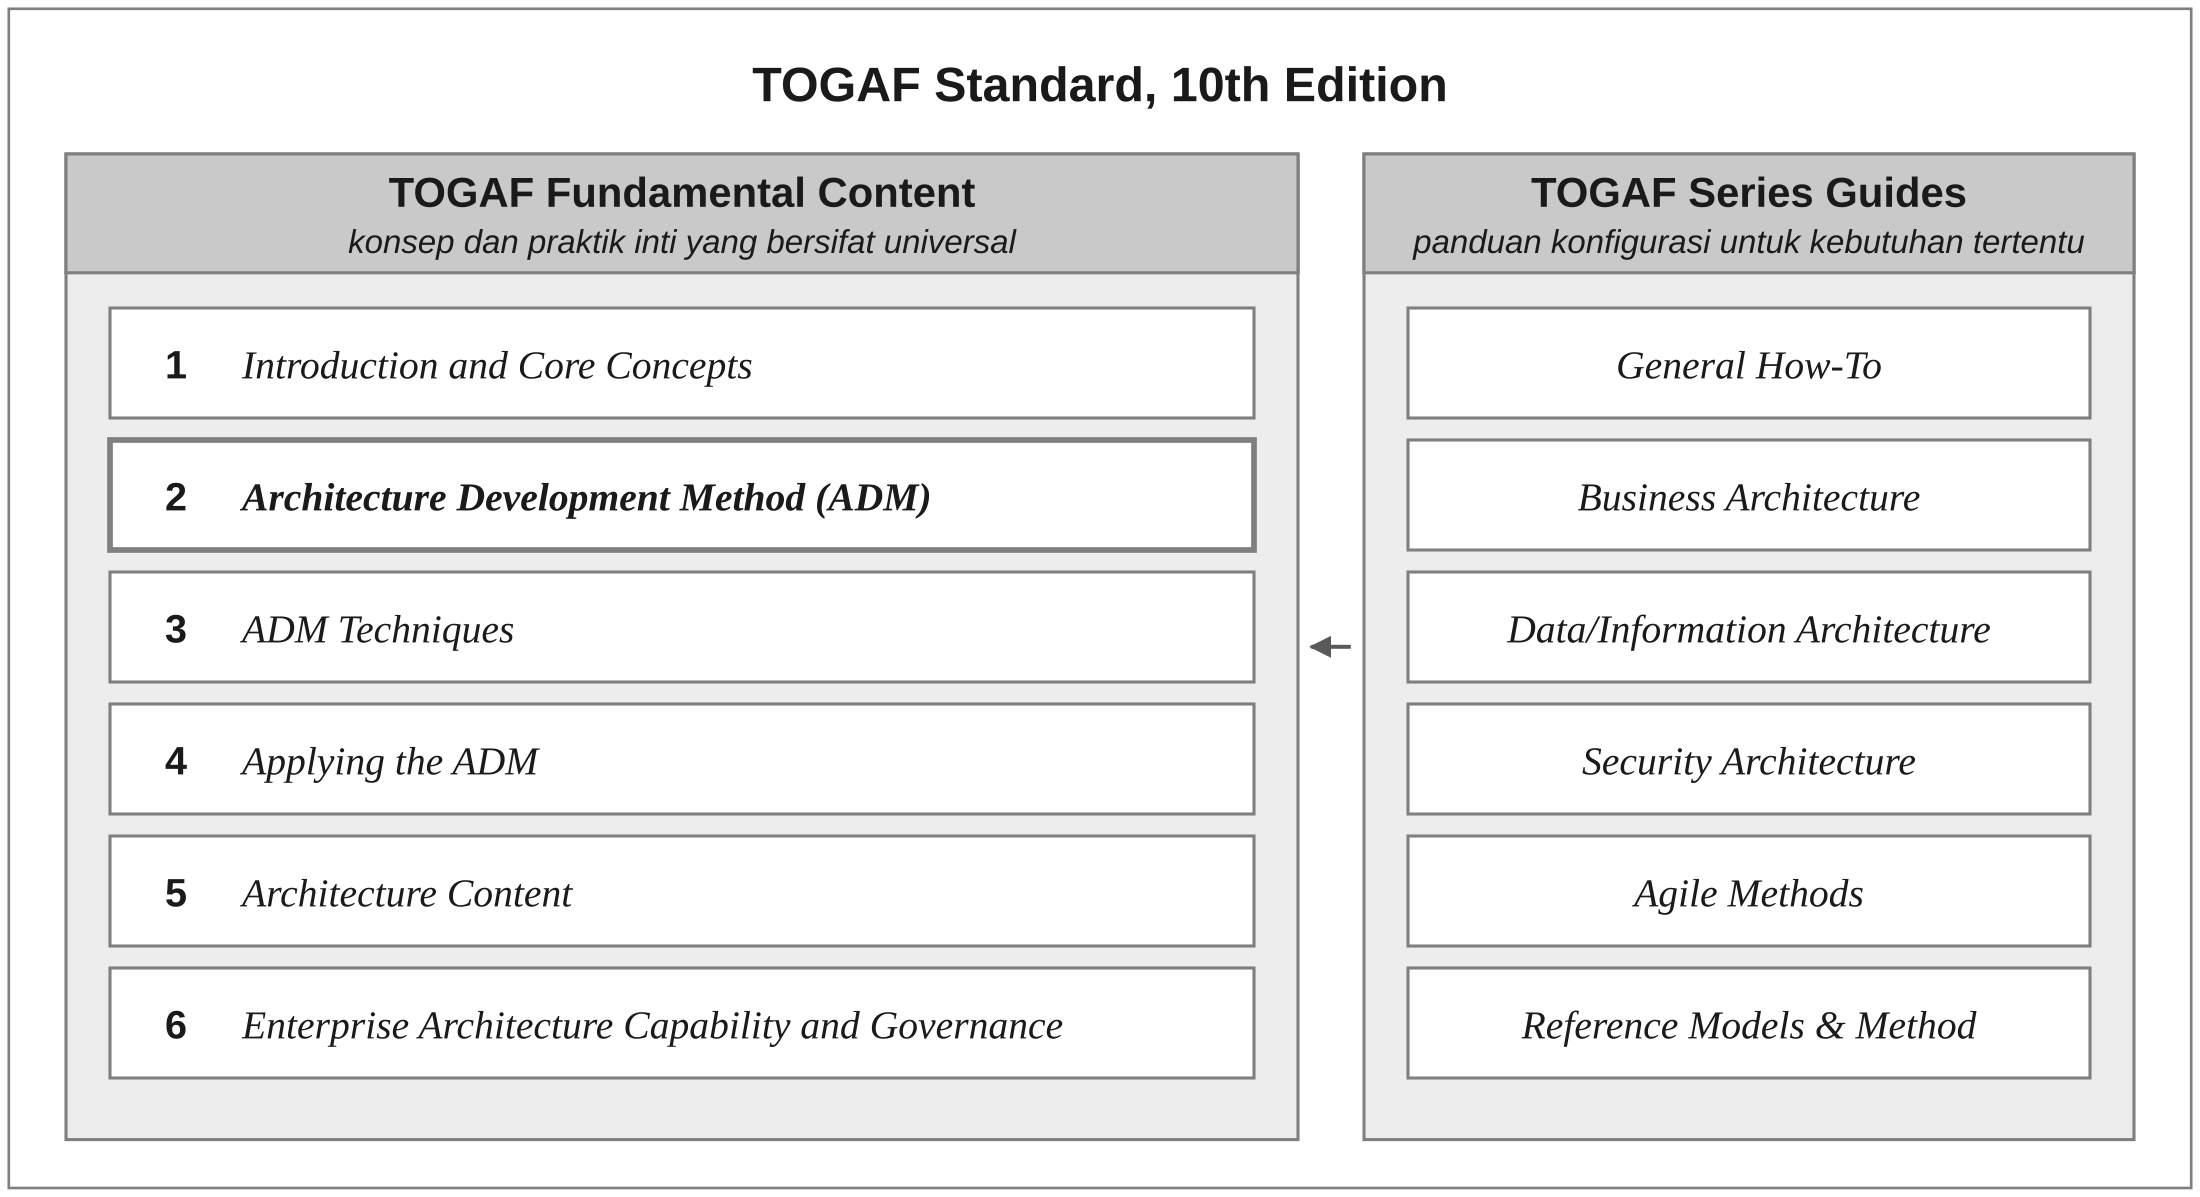
\includegraphics[width=1.00\linewidth,height=0.8\textheight,keepaspectratio]{images/Struktur TOGAF Standard 10th Edition.png}
\caption{Struktur \textit{TOGAF Standard, 10th Edition}}
\label{fig:II.13}
\end{figure}

Gambar~\ref{fig:II.13} menunjukkan bahwa \textit{TOGAF Fundamental Content} terdiri atas enam dokumen. Di antara keenam dokumen tersebut, \textit{Architecture Development Method} (ADM) merupakan inti TOGAF karena menyediakan proses yang teruji dan dapat diulang untuk mengembangkan arsitektur. Dokumen lainnya menopang ADM, yaitu teknik pendukung, panduan penerapan ADM melalui iterasi dan partisi arsitektur, kerangka konten arsitektur, serta pembentukan kapabilitas dan tata kelola EA \cite{TOGAF2022}. Adapun \textit{TOGAF Series Guides} menjabarkan konsep inti tersebut untuk kebutuhan tertentu, misalnya arsitektur bisnis, arsitektur data, arsitektur keamanan, dan metode \textit{agile}.

Selain dokumen tersebut, TOGAF memiliki beberapa komponen inti yang digunakan sepanjang pengembangan arsitektur, yaitu sebagai berikut \cite{TOGAF2022}:
\begin{enumerate}[label=\arabic*.]
\item \textit{Architecture Content Framework} dan \textit{Enterprise Metamodel}, yang menetapkan jenis keluaran arsitektur, yaitu \textit{deliverable}, artefak, dan \textit{building block}, beserta hubungan antarkeluaran tersebut.
\item \textit{Enterprise Continuum}, yang mengklasifikasikan aset arsitektur mulai dari yang bersifat generik hingga yang spesifik bagi organisasi.
\item \textit{Architecture Repository}, yang menyimpan seluruh keluaran arsitektur agar dapat digunakan ulang pada siklus berikutnya.
\item \textit{Architecture Capability} dan tata kelola arsitektur, yang memastikan praktik EA berjalan sebagai fungsi organisasi yang berkelanjutan.
\end{enumerate}

\subsection{\textit{Architecture Development Method} (ADM)}
\label{sec:II.5.2}
\begin{figure}[htbp]
\centering
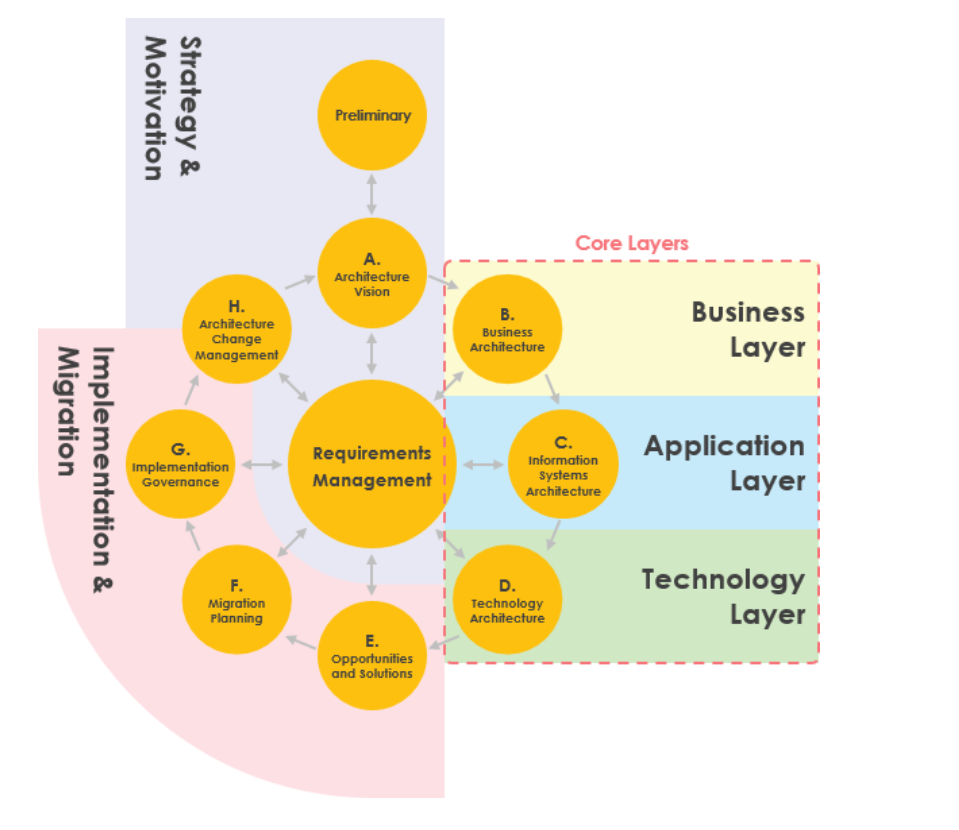
\includegraphics[width=0.79\linewidth,height=0.8\textheight,keepaspectratio]{images/Siklus TOGAF ADM.png}
\caption{Siklus TOGAF Architecture Development Method (ADM)}
\label{fig:II.14}
\end{figure}

ADM merupakan metode untuk mengembangkan dan mengelola siklus hidup EA, sekaligus inti dari TOGAF \cite{TOGAF2022}. ADM terdiri atas Fase \textit{Preliminary}, delapan fase pengembangan arsitektur, yaitu Fase A hingga Fase H, serta \textit{Requirements Management} yang berada di pusat siklus, sebagaimana ditunjukkan pada Gambar~\ref{fig:II.14}.

Gambar~\ref{fig:II.14} menunjukkan bahwa Fase \textit{Preliminary} menjadi titik masuk siklus, kemudian fase-fase pengembangan arsitektur dijalankan secara berurutan dari Fase A hingga Fase H. \textit{Requirements Management} merupakan fase yang berlangsung terus-menerus untuk memastikan setiap perubahan kebutuhan dikelola melalui tata kelola dan diteruskan ke seluruh fase \cite{TOGAF2022}. Tujuan setiap fase ADM disajikan pada Tabel~\ref{tab:II.3}.
\begingroup\small\setstretch{1.0}
\begin{longtable}{@{}>{\raggedright\arraybackslash}p{0.366\linewidth}>{\raggedright\arraybackslash}p{0.601\linewidth}@{}}
\caption{Fase TOGAF ADM dan Tujuannya}\label{tab:II.3}\\
\toprule
\textbf{Fase} & \textbf{Tujuan Utama}\\
\midrule
\endfirsthead
\multicolumn{2}{@{}l}{\small\itshape \tablename\ \thetable{} (lanjutan)}\\
\toprule
\textbf{Fase} & \textbf{Tujuan Utama}\\
\midrule
\endhead
\bottomrule
\endlastfoot
\textit{Preliminary} & Menetapkan kapabilitas arsitektur yang dibutuhkan organisasi, termasuk prinsip arsitektur, tata kelola, dan penyesuaian \textit{framework}.\\
A. \textit{Architecture Vision} & Menetapkan ruang lingkup, pemangku kepentingan, dan visi arsitektur, serta memperoleh persetujuan melalui \textit{Statement of Architecture Work}.\\
B. \textit{Business Architecture} & Mengembangkan arsitektur bisnis \textit{baseline} dan \textit{target} serta menganalisis kesenjangannya.\\
C. \textit{Information Systems Architectures} & Mengembangkan arsitektur data dan aplikasi \textit{baseline} dan \textit{target} serta menganalisis kesenjangannya.\\
D. \textit{Technology Architecture} & Mengembangkan arsitektur teknologi \textit{baseline} dan \textit{target} serta menganalisis kesenjangannya.\\
E. \textit{Opportunities and Solutions} & Mengidentifikasi paket pekerjaan dan arsitektur transisi untuk mewujudkan arsitektur \textit{target}.\\
F. \textit{Migration Planning} & Menyusun rencana implementasi dan migrasi yang rinci beserta prioritasnya.\\
G. \textit{Implementation Governance} & Mengawasi implementasi agar sesuai dengan arsitektur \textit{target}.\\
H. \textit{Architecture Change Management} & Mengelola perubahan arsitektur secara berkelanjutan setelah implementasi.\\
\textit{Requirements Management} & Mengelola kebutuhan arsitektur sepanjang siklus ADM.\\
\end{longtable}
\endgroup

ADM bersifat iteratif. Setiap iterasi memanfaatkan artefak dan kapabilitas yang dihasilkan pada iterasi sebelumnya serta menambah isi \textit{Architecture Repository}. Gambar~\ref{fig:II.14} juga menunjukkan pengelompokan fase ADM berdasarkan keterkaitannya dengan lapisan bahasa pemodelan ArchiMate \cite{ArchiMate2019}, yaitu sebagai berikut:
\begin{enumerate}[label=\arabic*.]
\item \textit{Strategy \& Motivation}, yang mencakup Fase \textit{Preliminary}, Fase A, \textit{Requirements Management}, dan sebagian Fase H. Kelompok ini menetapkan arah, prinsip, dan kebutuhan arsitektur.
\item \textit{Core Layers}, yang mencakup Fase B, C, dan D. Ketiga fase ini masing-masing merancang lapisan bisnis (\textit{Business Layer}), lapisan aplikasi (\textit{Application Layer}), dan lapisan teknologi (\textit{Technology Layer}).
\item \textit{Implementation \& Migration}, yang mencakup Fase E, F, G, dan sebagian Fase H. Kelompok ini merencanakan dan mengawal perwujudan arsitektur target.
\end{enumerate}

Pengelompokan tersebut sejalan dengan siklus iterasi yang disarankan TOGAF, yaitu iterasi kapabilitas arsitektur pada kelompok pertama, iterasi pengembangan arsitektur pada kelompok kedua, serta iterasi perencanaan transisi dan iterasi tata kelola arsitektur pada kelompok ketiga \cite{TOGAF2022}. Fase H berada pada dua kelompok karena fase ini mengelola perubahan arsitektur setelah implementasi sekaligus dapat memicu siklus ADM yang baru. Dalam penelitian ini, ADM digunakan sebagai dasar TOGAF Pertahanan Indonesia, dengan penerapan dari Fase \textit{Preliminary} hingga Fase \textit{Migration Planning}.

\subsection{Penyesuaian (\textit{Tailoring}) dan Modifikasi TOGAF}
\label{sec:II.5.3}

TOGAF menyatakan bahwa ADM merupakan metode generik, sehingga sering kali perlu dimodifikasi atau diperluas untuk memenuhi kebutuhan tertentu. Penyesuaian tersebut dapat mencakup urutan fase, integrasi dengan \textit{framework} lain, serta penyesuaian \textit{deliverable} dan artefak dengan kebutuhan organisasi. ADM bahkan dirancang dengan mempertimbangkan integrasi dengan \textit{framework} lain, termasuk \textit{framework} yang berfokus pada sektor tertentu, seperti pemerintahan dan pertahanan.

Penyesuaian TOGAF ditetapkan sejak Fase \textit{Preliminary} melalui tiga bentuk, yaitu sebagai berikut \cite{TOGAF2022}:
\begin{enumerate}[label=\arabic*.]
\item Penyesuaian terminologi, yaitu penggunaan istilah yang dipahami secara umum di lingkungan organisasi.
\item Penyesuaian proses, yaitu menghapus tugas yang telah dilakukan di tempat lain, menambahkan tugas khusus organisasi, serta menyelaraskan ADM dengan proses dan kerangka kerja lain yang berlaku.
\item Penyesuaian konten, yaitu menyesuaikan struktur dan klasifikasi konten arsitektur agar dapat mengadopsi kerangka konten lain dan memenuhi kebutuhan khusus organisasi.
\end{enumerate}

TOGAF juga menyediakan contoh perluasan melalui \textit{Series Guides}. Salah satunya adalah panduan integrasi risiko dan keamanan yang menambahkan aktivitas keamanan pada fase-fase ADM, tetapi tetap memperlakukan keamanan sebagai \textit{concern} lintas domain \cite{TOGAFRiskSecurity}.

Mekanisme tersebut menunjukkan bahwa TOGAF memberikan ruang modifikasi yang luas, tetapi tidak menyediakan muatan untuk sektor tertentu. Muatan pertahanan, seperti domain kapabilitas komando dan kendali, penautan arsitektur dengan doktrin pertahanan, dan interoperabilitas lintas matra, harus dirumuskan sendiri oleh organisasi. Penelitian ini memanfaatkan ruang tersebut melalui dua bentuk modifikasi, yaitu penyesuaian muatan lima fase (Δ) dan penambahan Fase \textit{C6ISR Architecture} (+).

\section{Perbandingan \textit{Framework} EA}
\label{sec:II.6}

Untuk menentukan \textit{framework} yang paling sesuai sebagai dasar modifikasi, maka dilakukan perbandingan antara DoDAF, NAF, MODAF, dan TOGAF berdasarkan beberapa aspek, sebagaimana ditunjukkan pada Tabel~\ref{tab:II.4}.
\begingroup\small\setstretch{1.0}
\begin{longtable}{@{}>{\raggedright\arraybackslash}p{0.157\linewidth}>{\raggedright\arraybackslash}p{0.180\linewidth}>{\raggedright\arraybackslash}p{0.180\linewidth}>{\raggedright\arraybackslash}p{0.180\linewidth}>{\raggedright\arraybackslash}p{0.180\linewidth}@{}}
\caption{Perbandingan \textit{Framework} EA}\label{tab:II.4}\\
\toprule
\textbf{Aspek} & \textbf{DoDAF} & \textbf{NAF} & \textbf{MODAF} & \textbf{TOGAF}\\
\midrule
\endfirsthead
\multicolumn{5}{@{}l}{\small\itshape \tablename\ \thetable{} (lanjutan)}\\
\toprule
\textbf{Aspek} & \textbf{DoDAF} & \textbf{NAF} & \textbf{MODAF} & \textbf{TOGAF}\\
\midrule
\endhead
\bottomrule
\endlastfoot
Pengembang & Departemen Pertahanan Amerika Serikat & NATO (\textit{Architecture Capability Team}, \textit{Digital Policy Committee}) & Kementerian Pertahanan Inggris & The Open Group\\
Versi dan status & 2.02 (2010), berlaku & 4.1 (2026), berlaku & 1.2.004 (2010), digantikan NAFv4 & \textit{10th Edition} (2022), berlaku\\
Orientasi utama & Mendukung keputusan dan proses inti DoD, seperti kapabilitas, anggaran, dan akuisisi & Standar arsitektur militer dan bisnis, terutama interoperabilitas NATO & Perencanaan pertahanan dan manajemen perubahan & EA generik lintas sektor\\
Struktur utama & 8 \textit{viewpoint}, 52 model, meta-model DM2 & \textit{Grid} 5 subjek × aspek perhatian; meta-model ArchiMate dan UAF & 7 \textit{viewpoint}; meta-model M3 & \textit{Fundamental Content} dan \textit{Series Guides}; 4 domain arsitektur\\
Metode pengembangan & 6 langkah yang bersifat umum & 8 tahap pada tingkat \textit{enterprise} dan proyek & Tidak menetapkan metode baku & ADM iteratif dengan \textit{Requirements Management} di pusat siklus\\
Penyesuaian & \textit{Fit-for-purpose}, tetapi terikat konvensi DoD & \textit{Viewpoint} dipilih sesuai \textit{concern}; mengikuti kebijakan NATO & Tidak lagi dikembangkan & Wajib sejak Fase \textit{Preliminary} (terminologi, proses, konten)\\
Muatan pertahanan & Kuat & Kuat & Kuat & Tidak tersedia\\
Keselarasan dengan Arsitektur SPBE & Perlu pemetaan ulang & Perlu pemetaan ulang & Perlu pemetaan ulang & Domain berpadanan (Tabel II.2)\\
\end{longtable}
\endgroup

Tabel~\ref{tab:II.4} menunjukkan perbedaan mendasar antara \textit{framework} EA pertahanan dan TOGAF. DoDAF dan MODAF menekankan apa yang harus dideskripsikan melalui \textit{viewpoint} dan model baku, sedangkan langkah pengembangannya bersifat umum. NAF telah memiliki metodologi, tetapi dirancang untuk lingkungan NATO. Ketiganya kuat dalam muatan pertahanan karena berakar pada \textit{C4ISR Architecture Framework}. Sebaliknya, TOGAF menekankan cara arsitektur dikembangkan secara bertahap melalui ADM dan bersifat netral terhadap sektor.

Bagi Kemhan RI, TOGAF memiliki tiga keunggulan. Pertama, ADM menyediakan metode yang iteratif dan lengkap, mulai dari penetapan kapabilitas arsitektur hingga perencanaan migrasi dan pengelolaan perubahan. Kedua, TOGAF dirancang untuk disesuaikan sejak Fase \textit{Preliminary}, sehingga modifikasi dapat dilakukan tanpa meninggalkan kerangka metodologisnya. Ketiga, domain TOGAF berpadanan dengan domain Arsitektur SPBE (Tabel~\ref{tab:II.2}), sehingga arsitektur yang dihasilkan dapat memenuhi kewajiban Kemhan RI sebagai instansi pemerintah. Selain itu, TOGAF tersedia secara terbuka untuk penggunaan akademik dan nonkomersial \cite{TOGAF2022}.

Namun, TOGAF tidak memiliki muatan pertahanan, seperti domain kapabilitas komando dan kendali, ISR, dan sistem tempur, sedangkan keamanan masih diperlakukan sebagai \textit{concern} lintas domain \cite{TOGAFRiskSecurity}. Pada titik inilah keunggulan \textit{framework} EA pertahanan menjadi relevan. Oleh karena itu, penelitian ini menggunakan TOGAF ADM sebagai kerangka metodologis utama dan menanamkan muatan pertahanan melalui model rujukan C6ISR.

\section{C6ISR}
\label{sec:II.7}

Subbab ini membahas C6ISR sebagai model rujukan kapabilitas pertahanan yang ditanamkan ke dalam TOGAF. Pembahasan meliputi evolusi konsep komando dan kendali hingga C6ISR, unsur-unsur C6ISR beserta keterpaduannya, serta konteks C6ISR dalam pertahanan Indonesia.

\subsection{Evolusi C2 hingga C6ISR}
\label{sec:II.7.1}

C6ISR merupakan hasil perkembangan bertahap dari konsep komando dan kendali (\textit{command and control}/C2). \textit{Command} adalah kewenangan untuk mengarahkan, mengoordinasikan, dan mengendalikan kekuatan militer, sedangkan \textit{control} adalah kewenangan komandan atas kegiatan organisasi bawahan atau organisasi lain, termasuk tanggung jawab untuk melaksanakan perintah. Fungsi C2 didukung oleh sistem informasi komando dan kendali (\textit{command and control information system}/C2IS), yaitu sistem perangkat keras dan perangkat lunak yang menyediakan informasi bagi pengambil keputusan untuk merencanakan, mengoordinasikan, dan mengelola operasi \cite{Todorovic2025}.

Seiring perkembangan teknologi, C2 diperluas dengan unsur komunikasi dan komputer menjadi C3 dan C4, kemudian dengan unsur intelijen, pengawasan, dan pengintaian menjadi C4ISR \cite{Petrovski2023,Todorovic2025}. Konsep C4ISR diformalkan pada tahun 1990-an melalui \textit{C4ISR Architecture Framework} yang kemudian menjadi dasar DoDAF \cite{C4ISRAWG1998}. Perkembangan berikutnya dipicu oleh meningkatnya peran ruang siber. Pada KTT Warsawa 2016, NATO mengakui ruang siber sebagai domain operasi yang harus dipertahankan, sebagaimana domain darat, laut, dan udara \cite{NATO2016Warsaw}. Unsur siber kemudian ditambahkan sehingga menjadi C5ISR, yang oleh Petrovski dkk. dirumuskan secara lebih spesifik sebagai \textit{cyber-defense} \cite{Petrovski2023}.

Tahap berikutnya adalah penambahan \textit{combat systems} sebagai unsur C keenam sehingga menjadi C6ISR \cite{Petrovski2023}. Penambahan ini dapat dipahami dari perbedaan C2IS dan sistem tempur terintegrasi. C2IS mengolah informasi medan operasi untuk mendukung keputusan, sedangkan sistem tempur terintegrasi memadukan sensor, fungsi C2, dan senjata untuk melaksanakan misi tempur \cite{Todorovic2025}. Contohnya adalah \textit{combat information center} pada kapal perang yang memadukan kemampuan C5ISR dengan sistem tempur \cite{Petrovski2023}. Dengan demikian, C6ISR melengkapi siklus operasi mulai dari pengindraan dan pengambilan keputusan hingga penindakan. Ringkasan evolusi tersebut disajikan pada Tabel~\ref{tab:II.5}.
\begingroup\small\setstretch{1.0}
\begin{longtable}{@{}>{\raggedright\arraybackslash}p{0.130\linewidth}>{\raggedright\arraybackslash}p{0.227\linewidth}>{\raggedright\arraybackslash}p{0.311\linewidth}>{\raggedright\arraybackslash}p{0.239\linewidth}@{}}
\caption{Evolusi Komando dan Kendali hingga C6ISR}\label{tab:II.5}\\
\toprule
\textbf{Kerangka} & \textbf{Unsur yang Ditambahkan} & \textbf{Fokus} & \textbf{Pendorong Utama}\\
\midrule
\endfirsthead
\multicolumn{4}{@{}l}{\small\itshape \tablename\ \thetable{} (lanjutan)}\\
\toprule
\textbf{Kerangka} & \textbf{Unsur yang Ditambahkan} & \textbf{Fokus} & \textbf{Pendorong Utama}\\
\midrule
\endhead
\bottomrule
\endlastfoot
\centering\arraybackslash C2 & \textit{Command}, \textit{Control} & Pelaksanaan kewenangan komandan untuk mengarahkan dan mengendalikan kekuatan & Kebutuhan dasar kepemimpinan dan pengendalian operasi\\
\centering\arraybackslash C3/C4 & \textit{Communications}, \textit{Computers} & Komunikasi dan komputasi untuk mendukung proses C2 & Perkembangan teknologi komunikasi dan komputer\\
\centering\arraybackslash C4ISR & \textit{Intelligence}, \textit{Surveillance}, \textit{Reconnaissance} & Integrasi pengumpulan informasi dan intelijen dengan fungsi C4 & Operasi berbasis jaringan dan formalisasi arsitektur pada 1990-an\\
\centering\arraybackslash C5ISR & \textit{Cyber-Defense} & Perlindungan jaringan, data, dan sistem dari serangan siber & Ruang siber diakui sebagai domain operasi\\
\centering\arraybackslash C6ISR & \textit{Combat Systems} & Integrasi sistem tempur dengan C2 sehingga keputusan diteruskan menjadi tindakan dan umpan balik & Kebutuhan melengkapi fungsi \textit{act} dalam siklus operasi\\
\end{longtable}
\endgroup

Tabel~\ref{tab:II.5} menunjukkan bahwa setiap tahap menambahkan unsur baru tanpa menghilangkan unsur sebelumnya. Meskipun demikian, C6ISR belum merupakan istilah doktrin yang baku. Todorović dkk. menyatakan bahwa berbagai istilah, seperti C3I, C4ISR, C4ISTAR, C5ISR, dan C6ISR, pada dasarnya merujuk pada konsep yang sama \cite{Todorovic2025}. Oleh karena itu, penelitian ini menetapkan C6ISR sebagai definisi operasional yang mencakup kapabilitas terintegrasi \textit{Command}, \textit{Control}, \textit{Communications}, \textit{Computers}, \textit{Cyber-Defense}, \textit{Combat Systems}, \textit{Intelligence}, \textit{Surveillance}, dan \textit{Reconnaissance}.

\subsection{Unsur-Unsur C6ISR}
\label{sec:II.7.2}

Petrovski dkk. menjelaskan fungsi setiap unsur C6ISR, sebagaimana dirangkum pada Tabel~\ref{tab:II.6} \cite{Petrovski2023}.
\begingroup\small\setstretch{1.0}
\begin{longtable}{@{}>{\raggedright\arraybackslash}p{0.276\linewidth}>{\raggedright\arraybackslash}p{0.690\linewidth}@{}}
\caption{Unsur-Unsur C6ISR dan Fungsinya}\label{tab:II.6}\\
\toprule
\textbf{Unsur} & \textbf{Fungsi}\\
\midrule
\endfirsthead
\multicolumn{2}{@{}l}{\small\itshape \tablename\ \thetable{} (lanjutan)}\\
\toprule
\textbf{Unsur} & \textbf{Fungsi}\\
\midrule
\endhead
\bottomrule
\endlastfoot
\textit{Command} & Mengambil keputusan strategis dan merencanakan operasi.\\
\textit{Control} & Memantau dan mengendalikan sensor, komunikasi, dan pengolahan data secara \textit{real-time}.\\
\textit{Communications} & Menyediakan pertukaran suara, data, dan video antarunit dan pusat komando melalui satelit, radio, dan jaringan optik.\\
\textit{Computers} & Mengolah dan menganalisis data dari berbagai sensor secara cepat, termasuk dengan kecerdasan buatan.\\
\textit{Cyber-Defense} & Melindungi sistem dari serangan siber melalui deteksi, pencegahan, dan respons.\\
\textit{Combat Systems} & Mendukung perencanaan, pelaksanaan, dan pengendalian operasi tempur oleh berbagai satuan dan platform.\\
\textit{Intelligence} & Mengumpulkan, menganalisis, dan menafsirkan data yang dibutuhkan untuk mengelola operasi.\\
\textit{Surveillance} & Memantau aktivitas dan situasi di medan operasi.\\
\textit{Reconnaissance} & Mengumpulkan dan menganalisis informasi untuk mengenali ancaman, kekuatan lawan, dan kondisi medan.\\
\end{longtable}
\endgroup

Unsur-unsur tersebut tidak bekerja secara terpisah, melainkan membentuk satu siklus operasi, sebagaimana ditunjukkan pada Gambar~\ref{fig:II.15}.
\begin{figure}[htbp]
\centering
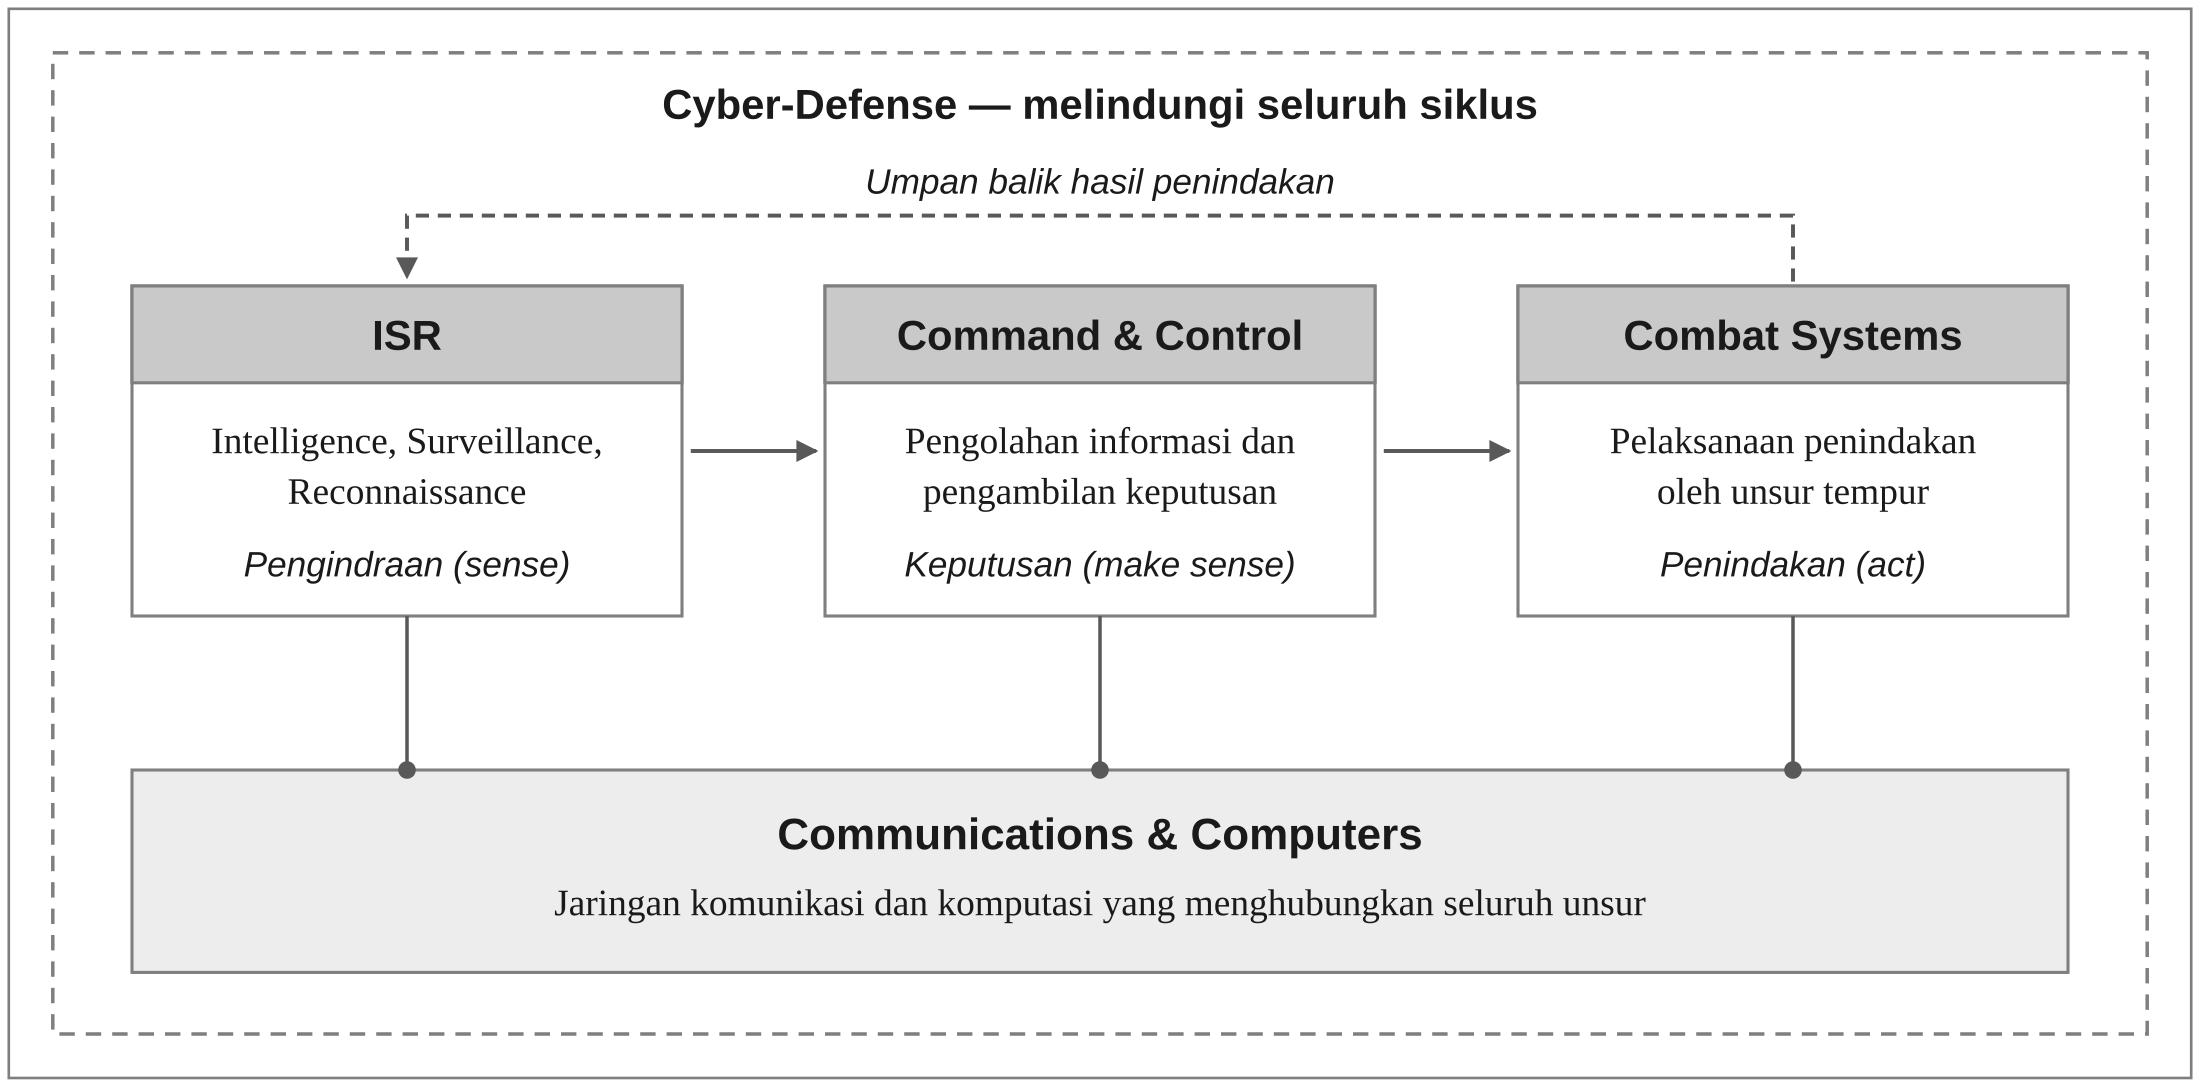
\includegraphics[width=1.00\linewidth,height=0.8\textheight,keepaspectratio]{images/Model Konseptual Keterpaduan C6ISR.png}
\caption{Model Konseptual Keterpaduan Unsur C6ISR}
\label{fig:II.15}
\end{figure}

Gambar~\ref{fig:II.15} menunjukkan bahwa unsur ISR berperan sebagai pengindraan (\textit{sense}), unsur komando dan kendali mengolah informasi menjadi keputusan (\textit{make sense}), dan \textit{combat systems} melaksanakan penindakan (\textit{act}) yang hasilnya menjadi umpan balik bagi pengindraan berikutnya \cite{USDoD2022}. \textit{Communications} dan \textit{computers} menjadi tulang punggung yang menghubungkan ketiga unsur tersebut, sedangkan \textit{cyber-defense} melindungi seluruh siklus. Karena efektivitas operasi ditentukan oleh keterpaduan antarunsur, C6ISR perlu dirancang sebagai satu kesatuan arsitektur, bukan sebagai sistem yang terpisah. Hal ini menjadi alasan C6ISR ditetapkan sebagai fase arsitektur tersendiri dalam TOGAF Pertahanan Indonesia.

Integrasi \textit{combat systems} juga menuntut pengendalian penggunaan kekuatan yang jelas. Kebijakan Departemen Pertahanan Amerika Serikat mensyaratkan sistem senjata otonom dan semi-otonom dirancang agar komandan dan operator tetap dapat menerapkan pertimbangan manusia yang memadai dalam penggunaan kekuatan \cite{DoDD300009}. Prinsip tersebut relevan karena otomasi dan kecerdasan buatan dapat mempercepat keputusan, tetapi tidak menghilangkan tanggung jawab manusia dalam keputusan penindakan.

\subsection{C6ISR dalam Konteks Pertahanan Indonesia}
\label{sec:II.7.3}

Di Indonesia, konsep yang serupa dengan C4ISR telah dikenal dengan istilah K4IPP. Permenhan Nomor 8 Tahun 2016 mendefinisikan K4IPP sebagai sistem yang memadukan dan menyinergikan unsur komando, kendali, komunikasi, komputerisasi, informasi, pengamatan, dan pengintaian guna meningkatkan kualitas komando dan pengendalian pimpinan Hankam/TNI kepada unsur pelaksana maupun sistem senjata secara cepat dan tepat \cite{Permenhan8Tahun2016}. Peraturan tersebut juga membagi penyelenggaraan sistem komunikasi menjadi tingkat Kemhan, sistem komunikasi strategis oleh Mabes TNI, dan sistem komunikasi taktis oleh setiap angkatan \cite{Permenhan8Tahun2016}.

Istilah C6ISR juga telah digunakan dalam kajian di lingkungan Kemhan RI. Kajian Ditjen Pothan Kemhan menyebutkan bahwa pembentukan holding BUMN industri pertahanan diharapkan mampu mengintegrasikan C6ISR pada tiga matra TNI dalam penerapan \textit{network centric warfare}. Kajian tersebut juga mengidentifikasi ketergantungan pada satelit sebagai tantangan, khususnya terkait kerahasiaan dan potensi sabotase apabila belum terdapat kemandirian satelit nasional \cite{Dwipratama2023}. Pada unsur \textit{cyber-defense}, Pedoman Pertahanan Siber mengidentifikasi ancaman terhadap perangkat keras, perangkat lunak, serta data dan informasi pertahanan \cite{Permenhan82Tahun2014}.

Uraian tersebut menunjukkan tiga hal. Pertama, unsur-unsur C6ISR telah memiliki landasan dalam regulasi dan kajian pertahanan Indonesia. Kedua, penyelenggaraannya masih terbagi per tingkat dan per matra, sejalan dengan permasalahan silo pada lapisan operasional. Ketiga, keterpaduan C6ISR membutuhkan acuan arsitektur yang menautkan kebijakan Kemhan RI dengan kebutuhan operasional TNI. Dalam penelitian ini, C6ISR dirancang dari sudut pandang Kemhan RI sebagai penyelenggara kebijakan dan standar, sedangkan komando dan pengendalian operasional tetap berada pada Mabes TNI.

\section{Penelitian Terkait}
\label{sec:II.8}

Subbab ini menguraikan dua kelompok penelitian terkait, yaitu penelitian EA di sektor pertahanan dan penelitian modifikasi TOGAF untuk domain khusus. Kedua kelompok penelitian tersebut kemudian dibandingkan untuk merumuskan kesenjangan penelitian dan posisi penelitian ini.

\subsection{EA di Sektor Pertahanan}
\label{sec:II.8.1}

Framework EA pertahanan kuat dalam deskripsi arsitektur, tetapi langkah pengembangannya bersifat umum. Oleh karena itu, sejumlah penelitian memadukan framework pertahanan dengan TOGAF. Dandashi dkk. menyatakan bahwa TOGAF dan DoDAF saling melengkapi karena TOGAF berfokus pada metode pengembangan arsitektur, sedangkan DoDAF berfokus pada deskripsi arsitektur melalui sekumpulan \textit{view}. Dalam paduan tersebut, ADM digunakan sebagai metode dan setiap produk DoDAF dipetakan ke fase ADM, misalnya AV-1 dan OV-1 pada Fase Preliminary dan Fase A, serta model operasional OV-1 hingga OV-6 pada Fase B \cite{Dandashi2006}.

Paduan serupa diterapkan oleh Angkatan Bersenjata Norwegia. Jørgensen dkk. melaporkan bahwa organisasi tersebut menggunakan TOGAF sebagai metode pengembangan dan NAF sebagai metamodel serta struktur konten arsitektur. Keduanya memerlukan penyesuaian yang cukup besar agar dapat digunakan bersama. Penyesuaian tersebut dilakukan melalui pemetaan rinci antara kerangka konten TOGAF 9 dan NAF, DoDAF, serta MODAF, yang kemudian diimplementasikan dalam repositori arsitektur militer nasional dan diterapkan mulai dari peta kapabilitas hingga interoperabilitas sistem dan akuisisi \cite{Jorgensen2011}.

Penelitian lain menerapkan framework pertahanan pada objek yang lebih spesifik. Zain dkk. menggunakan DoDAF untuk merancang arsitektur \textit{as-is} dan \textit{to-be} pada DefTech, sebuah perusahaan industri pertahanan Malaysia, dengan menambahkan pencegahan kebocoran data untuk memperkuat keamanan siber \cite{Zain2023}. Fang dkk. memadukan pola keputusan (\textit{decision pattern}) dengan pemodelan DoDAF untuk menghasilkan alternatif arsitektur \textit{system of systems}, yang didemonstrasikan pada sistem peperangan antikapal selam \cite{Fang2024}. Lundberg dkk. memperluas NAF dengan panduan navigasi dan tujuh \textit{method chunk} untuk menentukan titik awal dan urutan pemodelan sistem C2, yang didemonstrasikan pada integrasi kapabilitas ISR ke dalam sistem C2 \cite{Lundberg2026}.

Penelitian-penelitian tersebut menunjukkan dua pola. Pertama, TOGAF telah digunakan di sektor pertahanan, tetapi sebagai metode yang dipadukan dengan framework pertahanan melalui pemetaan artefak dan metamodel. Kedua, penelitian yang memuat kapabilitas C2 dan ISR dilakukan pada tingkat sistem dengan framework pertahanan, bukan pada tingkat EA kementerian. Belum ditemukan penelitian yang menanamkan kapabilitas operasional pertahanan ke dalam siklus ADM.

\subsection{Modifikasi TOGAF untuk Domain Khusus}
\label{sec:II.8.2}

TOGAF menyediakan ruang penyesuaian terminologi, proses, dan konten. Ruang tersebut telah dimanfaatkan oleh sejumlah penelitian untuk menyesuaikan TOGAF dengan domain tertentu. Setyadi memodifikasi TOGAF untuk membangun \textit{architecture framework} e-government pada pemerintah kabupaten/kota. Modifikasi dilakukan pada langkah-langkah dalam fase ADM dan artefak yang dihasilkan, dengan dimensi Pemeringkatan e-Government Indonesia (PeGI) sebagai tolok ukur yang ditelusuri melalui analisis tematik \cite{Setyadi2015}.

Pada sektor statistik, BPS mengadopsi TOGAF ADM sebagai metodologi EA, tetapi menyederhanakan sembilan fase ADM menjadi lima tahap, yaitu \textit{Initiation}, \textit{Establishment}, \textit{Conceptualization}, \textit{Realization}, dan \textit{Observation}, agar lebih modular dan dapat direplikasi di lingkungan BPS. Arsitektur target disusun dengan mengadopsi GAMSO dan CSPA sebagai arsitektur rujukan statistik \cite{Virantina2020}. Pada domain \textit{smart city}, Bastidas dkk. mengevaluasi penerapan TOGAF pada layanan Kota Limerick, Irlandia. Penelitian tersebut menemukan bahwa TOGAF belum memuat prinsip, pemangku kepentingan, dan konsep domain kota, serta kurang rinci dalam memodelkan sensor dan \textit{gateway}. Oleh karena itu, penelitian tersebut merekomendasikan modifikasi atau perluasan ADM dan metamodelnya dengan konsep domain \textit{smart city} \cite{Bastidas2023}.

Penelitian-penelitian tersebut menunjukkan tiga bentuk modifikasi TOGAF, yaitu penyesuaian langkah dan artefak, penyederhanaan fase, serta penanaman model rujukan atau konsep domain. Pada ketiga bentuk tersebut, muatan domain ditanamkan ke dalam fase yang sudah ada dan tidak ada fase yang didedikasikan untuk domain tersebut. Penelitian ini mengikuti bentuk ketiga, tetapi mengembangkannya dengan menjadikan model rujukan domain, yaitu C6ISR, sebagai fase arsitektur tersendiri.

\subsection{Kesenjangan Penelitian (\textit{Research Gap})}
\label{sec:II.8.3}

Penelitian terkait pada Subbab~\ref{sec:II.8.1} dan II.8.2 dibandingkan berdasarkan lima kriteria yang diturunkan dari tujuan penelitian ini, yaitu K1 objek pada sektor pertahanan, K2 penggunaan TOGAF ADM sebagai metode, K3 modifikasi ADM, K4 muatan kapabilitas komando, kendali, dan ISR, serta K5 konteks instansi pemerintah Indonesia. Hasil perbandingan disajikan pada Tabel~\ref{tab:II.7}.
\begingroup\small\setstretch{1.0}
\begin{longtable}{@{}>{\raggedright\arraybackslash}p{0.245\linewidth}>{\raggedright\arraybackslash}p{0.221\linewidth}>{\raggedright\arraybackslash}p{0.070\linewidth}>{\raggedright\arraybackslash}p{0.070\linewidth}>{\raggedright\arraybackslash}p{0.070\linewidth}>{\raggedright\arraybackslash}p{0.070\linewidth}>{\raggedright\arraybackslash}p{0.070\linewidth}@{}}
\caption{Pemetaan Penelitian Terkait}\label{tab:II.7}\\
\toprule
\textbf{Penelitian} & \textbf{Objek/Domain} & \textbf{K1} & \textbf{K2} & \textbf{K3} & \textbf{K4} & \textbf{K5}\\
\midrule
\endfirsthead
\multicolumn{7}{@{}l}{\small\itshape \tablename\ \thetable{} (lanjutan)}\\
\toprule
\textbf{Penelitian} & \textbf{Objek/Domain} & \textbf{K1} & \textbf{K2} & \textbf{K3} & \textbf{K4} & \textbf{K5}\\
\midrule
\endhead
\bottomrule
\endlastfoot
Dandashi dkk. (2006) \cite{Dandashi2006} & Pertahanan (DoD) & \centering\arraybackslash √ & \centering\arraybackslash √ & \centering\arraybackslash √ & \centering\arraybackslash – & \centering\arraybackslash –\\
Jørgensen dkk. (2011) \cite{Jorgensen2011} & Angkatan Bersenjata Norwegia & \centering\arraybackslash √ & \centering\arraybackslash √ & \centering\arraybackslash √ & \centering\arraybackslash – & \centering\arraybackslash –\\
Setyadi (2015) \cite{Setyadi2015} & E-government kabupaten/kota & \centering\arraybackslash – & \centering\arraybackslash √ & \centering\arraybackslash √ & \centering\arraybackslash – & \centering\arraybackslash √\\
Virantina dkk. (2020) \cite{Virantina2020} & Statistik (BPS) & \centering\arraybackslash – & \centering\arraybackslash √ & \centering\arraybackslash √ & \centering\arraybackslash – & \centering\arraybackslash √\\
Zain dkk. (2023) \cite{Zain2023} & Industri pertahanan & \centering\arraybackslash √ & \centering\arraybackslash – & \centering\arraybackslash – & \centering\arraybackslash – & \centering\arraybackslash –\\
Bastidas dkk. (2023) \cite{Bastidas2023} & \textit{Smart city} & \centering\arraybackslash – & \centering\arraybackslash √ & \centering\arraybackslash – & \centering\arraybackslash – & \centering\arraybackslash –\\
Fang dkk. (2024) \cite{Fang2024} & \textit{System of systems} pertahanan & \centering\arraybackslash √ & \centering\arraybackslash – & \centering\arraybackslash – & \centering\arraybackslash – & \centering\arraybackslash –\\
Lundberg dkk. (2026) \cite{Lundberg2026} & Sistem C2 & \centering\arraybackslash √ & \centering\arraybackslash – & \centering\arraybackslash – & \centering\arraybackslash √ & \centering\arraybackslash –\\
Penelitian ini & Pertahanan (Kemhan RI) & \centering\arraybackslash √ & \centering\arraybackslash √ & \centering\arraybackslash √ & \centering\arraybackslash √ & \centering\arraybackslash √\\
\end{longtable}
\endgroup

Keterangan: √ = terpenuhi; – = tidak terpenuhi.

Tabel~\ref{tab:II.7} menunjukkan bahwa belum terdapat penelitian yang memenuhi kelima kriteria secara bersamaan. Kesenjangan penelitian yang teridentifikasi adalah sebagai berikut.
\begin{enumerate}[label=\arabic*.]
\item Penelitian EA pertahanan yang menggunakan TOGAF memadukannya dengan framework pertahanan melalui pemetaan artefak dan metamodel, tetapi belum menanamkan kapabilitas operasional pertahanan ke dalam siklus ADM.
\item Penelitian yang memuat kapabilitas C2 dan ISR dilakukan pada tingkat sistem dengan framework pertahanan, sehingga belum terhubung dengan EA pada tingkat kementerian.
\item Modifikasi TOGAF untuk domain khusus, termasuk pada instansi pemerintah Indonesia, menanamkan muatan domain ke dalam fase yang sudah ada dan belum diterapkan pada sektor pertahanan.
\end{enumerate}

Penelitian ini mengisi kesenjangan tersebut melalui TOGAF Pertahanan Indonesia, yaitu modifikasi TOGAF ADM yang menyesuaikan muatan lima fase (Δ) dan menambahkan Fase C6ISR Architecture (+). Framework tersebut kemudian diterapkan pada Kemhan RI dengan tetap selaras dengan Arsitektur SPBE. Rancangan modifikasi tersebut diuraikan pada Bab III.
